\documentclass[]{article}
\usepackage{lmodern}
\usepackage{amssymb,amsmath}
\usepackage{ifxetex,ifluatex}
\usepackage{fixltx2e} % provides \textsubscript
\ifnum 0\ifxetex 1\fi\ifluatex 1\fi=0 % if pdftex
  \usepackage[T1]{fontenc}
  \usepackage[utf8]{inputenc}
\else % if luatex or xelatex
  \ifxetex
    \usepackage{mathspec}
  \else
    \usepackage{fontspec}
  \fi
  \defaultfontfeatures{Ligatures=TeX,Scale=MatchLowercase}
\fi
% use upquote if available, for straight quotes in verbatim environments
\IfFileExists{upquote.sty}{\usepackage{upquote}}{}
% use microtype if available
\IfFileExists{microtype.sty}{%
\usepackage{microtype}
\UseMicrotypeSet[protrusion]{basicmath} % disable protrusion for tt fonts
}{}
\usepackage[margin=1in]{geometry}
\usepackage{hyperref}
\hypersetup{unicode=true,
            pdftitle={Credit Card Fraud Detection Capstone Project - Report},
            pdfauthor={Alessandro Corradini - Harvard Data Science Professional},
            pdfborder={0 0 0},
            breaklinks=true}
\urlstyle{same}  % don't use monospace font for urls
\usepackage{graphicx,grffile}
\makeatletter
\def\maxwidth{\ifdim\Gin@nat@width>\linewidth\linewidth\else\Gin@nat@width\fi}
\def\maxheight{\ifdim\Gin@nat@height>\textheight\textheight\else\Gin@nat@height\fi}
\makeatother
% Scale images if necessary, so that they will not overflow the page
% margins by default, and it is still possible to overwrite the defaults
% using explicit options in \includegraphics[width, height, ...]{}
\setkeys{Gin}{width=\maxwidth,height=\maxheight,keepaspectratio}
\IfFileExists{parskip.sty}{%
\usepackage{parskip}
}{% else
\setlength{\parindent}{0pt}
\setlength{\parskip}{6pt plus 2pt minus 1pt}
}
\setlength{\emergencystretch}{3em}  % prevent overfull lines
\providecommand{\tightlist}{%
  \setlength{\itemsep}{0pt}\setlength{\parskip}{0pt}}
\setcounter{secnumdepth}{5}
% Redefines (sub)paragraphs to behave more like sections
\ifx\paragraph\undefined\else
\let\oldparagraph\paragraph
\renewcommand{\paragraph}[1]{\oldparagraph{#1}\mbox{}}
\fi
\ifx\subparagraph\undefined\else
\let\oldsubparagraph\subparagraph
\renewcommand{\subparagraph}[1]{\oldsubparagraph{#1}\mbox{}}
\fi

%%% Use protect on footnotes to avoid problems with footnotes in titles
\let\rmarkdownfootnote\footnote%
\def\footnote{\protect\rmarkdownfootnote}

%%% Change title format to be more compact
\usepackage{titling}

% Create subtitle command for use in maketitle
\providecommand{\subtitle}[1]{
  \posttitle{
    \begin{center}\large#1\end{center}
    }
}

\setlength{\droptitle}{-2em}

  \title{Credit Card Fraud Detection Capstone Project - Report}
    \pretitle{\vspace{\droptitle}\centering\huge}
  \posttitle{\par}
    \author{Alessandro Corradini - Harvard Data Science Professional}
    \preauthor{\centering\large\emph}
  \postauthor{\par}
      \predate{\centering\large\emph}
  \postdate{\par}
    \date{May 24, 2019}

\usepackage{booktabs}
\usepackage{longtable}
\usepackage{array}
\usepackage{multirow}
\usepackage{wrapfig}
\usepackage{float}
\usepackage{colortbl}
\usepackage{pdflscape}
\usepackage{tabu}
\usepackage{threeparttable}
\usepackage{threeparttablex}
\usepackage[normalem]{ulem}
\usepackage{makecell}
\usepackage{xcolor}

\begin{document}
\maketitle
\begin{abstract}
This is the final assignment for the Harvard Data Science Professional
Program taught by the famous Prof.~of Biostatistics Rafael Irizarry from
Harvard University. In this capstone project, we have to choose a
dataset and we have to analyze it and perform our machine learning tasks
in complete autonomy without external help.
\end{abstract}

{
\setcounter{tocdepth}{2}
\tableofcontents
}
\newpage

\hypertarget{executive-summary}{%
\section{Executive Summary}\label{executive-summary}}

It is important that credit card companies are able to recognize
fraudulent credit card transactions so that customers are not charged
for items that they did not purchase. The datasets contains transactions
made by credit cards in September 2013 by european cardholders.

Due to imbalancing nature of the data, many observations could be
predicted as False Negative, in this case Legal Transactions instead of
Fraudolent Transaction. For example, a model that predict always
\textbf{0} (Legal) can archieve an Accuracy of \textbf{99.8}. For that
reason, the metric used for measuring the score is the \textbf{Area
Under The Precision-Recall Curve (AUCPR)} instead of the traditional AUC
curve. A desiderable result is an AUCPR at least greater than
\textbf{0.85}.

For archieving the task of classifying credit card fraud detection, they
are trained several algorithms such as Naive Bayes Classifier, KNN, SVM,
Random Forest, GBM, XGBoost and LightGBM.

In this analysis, a XGBoost Model is capable of an AUCPR of
\textbf{0.8623} and this is great!

\hypertarget{exploratory-data-analysis}{%
\section{Exploratory Data Analysis}\label{exploratory-data-analysis}}

\hypertarget{the-dataset}{%
\subsection{The Dataset}\label{the-dataset}}

This dataset presents transactions that occurred in two days, where we
have \textbf{492 frauds} out of \textbf{284,807 transactions}. The
dataset is highly unbalanced, the positive class (frauds) account for
0.172\% of all transactions.

The dataset contains only numerical input variables which are the result
of a PCA transformation. Unfortunately, due to confidentiality issues,
we cannot provide the original features and more background information
about the data. Features V1, V2, \ldots{} V28 are the principal
components obtained with PCA, the only features which have not been
transformed with PCA are `Time' and `Amount'.

\textbf{Source}

\url{https://www.kaggle.com/mlg-ulb/creditcardfraud}

\textbf{Dimensions}

\begin{table}[H]
\centering\begingroup\fontsize{10}{12}\selectfont

\begin{tabular}{r|r}
\hline
Length & Columns\\
\hline
284807 & 31\\
\hline
\end{tabular}
\endgroup{}
\end{table}

\textbf{Imbalanced Dataset}

This is a very imbalanced dataset. It means that there are few rows that
represent a class. In this case, only \textbf{492} transactions are
frauds, represented by \textbf{1} and \textbf{284315} are not,
represented by \textbf{0}.

\begin{center}\includegraphics{Credit_Card_Fraud_Detection_Project_Report_files/figure-latex/unnamed-chunk-6-1} \end{center}

\begin{table}[H]
\centering\begingroup\fontsize{10}{12}\selectfont

\begin{tabular}{r|r}
\hline
Class & Count\\
\hline
0 & 284315\\
\hline
1 & 492\\
\hline
\end{tabular}
\endgroup{}
\end{table}
\newpage

\textbf{Missing Values}

As the table below suggests, there aren't missing values in this
dataframe.

\begin{table}[H]
\centering\begingroup\fontsize{10}{12}\selectfont

\begin{tabular}{l|r}
\hline
  & Missing Values\\
\hline
Time & 0\\
\hline
V1 & 0\\
\hline
V2 & 0\\
\hline
V3 & 0\\
\hline
V4 & 0\\
\hline
V5 & 0\\
\hline
V6 & 0\\
\hline
V7 & 0\\
\hline
V8 & 0\\
\hline
V9 & 0\\
\hline
V10 & 0\\
\hline
V11 & 0\\
\hline
V12 & 0\\
\hline
V13 & 0\\
\hline
V14 & 0\\
\hline
V15 & 0\\
\hline
V16 & 0\\
\hline
V17 & 0\\
\hline
V18 & 0\\
\hline
V19 & 0\\
\hline
V20 & 0\\
\hline
V21 & 0\\
\hline
V22 & 0\\
\hline
V23 & 0\\
\hline
V24 & 0\\
\hline
V25 & 0\\
\hline
V26 & 0\\
\hline
V27 & 0\\
\hline
V28 & 0\\
\hline
Amount & 0\\
\hline
Class & 0\\
\hline
\end{tabular}
\endgroup{}
\end{table}

\textbf{First 10 Rows of \texttt{creditcard} dataset}

\begin{table}[H]
\centering\begingroup\fontsize{10}{12}\selectfont

\begin{tabular}{r|r|r|r|r|r|r|r|r}
\hline
Time & V1 & V2 & V3 & V4 & V5 & V28 & Amount & Class\\
\hline
0 & -1.3598071 & -0.0727812 & 2.5363467 & 1.3781552 & -0.3383208 & -0.0210531 & 149.62 & 0\\
\hline
0 & 1.1918571 & 0.2661507 & 0.1664801 & 0.4481541 & 0.0600176 & 0.0147242 & 2.69 & 0\\
\hline
1 & -1.3583541 & -1.3401631 & 1.7732093 & 0.3797796 & -0.5031981 & -0.0597518 & 378.66 & 0\\
\hline
1 & -0.9662717 & -0.1852260 & 1.7929933 & -0.8632913 & -0.0103089 & 0.0614576 & 123.50 & 0\\
\hline
2 & -1.1582331 & 0.8777368 & 1.5487178 & 0.4030339 & -0.4071934 & 0.2151531 & 69.99 & 0\\
\hline
2 & -0.4259659 & 0.9605230 & 1.1411093 & -0.1682521 & 0.4209869 & 0.0810803 & 3.67 & 0\\
\hline
4 & 1.2296576 & 0.1410035 & 0.0453708 & 1.2026127 & 0.1918810 & 0.0051678 & 4.99 & 0\\
\hline
7 & -0.6442694 & 1.4179635 & 1.0743804 & -0.4921990 & 0.9489341 & -1.0853392 & 40.80 & 0\\
\hline
7 & -0.8942861 & 0.2861572 & -0.1131922 & -0.2715261 & 2.6695987 & 0.1424043 & 93.20 & 0\\
\hline
9 & -0.3382618 & 1.1195934 & 1.0443666 & -0.2221873 & 0.4993608 & 0.0830756 & 3.68 & 0\\
\hline
\end{tabular}
\endgroup{}
\end{table}
\newpage

\textbf{Frauds Amount Distributions}

Small amount of money, less or equal of one dollar are scammed more
frequently.

\begin{center}\includegraphics{Credit_Card_Fraud_Detection_Project_Report_files/figure-latex/unnamed-chunk-10-1} \end{center}

\begin{table}[H]
\centering\begingroup\fontsize{10}{12}\selectfont

\begin{tabular}{r|r}
\hline
Amount & count\\
\hline
1.00 & 113\\
\hline
0.00 & 27\\
\hline
99.99 & 27\\
\hline
0.76 & 17\\
\hline
0.77 & 10\\
\hline
0.01 & 5\\
\hline
2.00 & 4\\
\hline
3.79 & 4\\
\hline
0.68 & 3\\
\hline
1.10 & 3\\
\hline
\end{tabular}
\endgroup{}
\end{table}
\newpage

\textbf{Frauds over Time Distribution}

There aren't correlation between \texttt{time} and frauds. A fraud can
happen anytime. It seems not particularly useful for the modelling
phase. The correlation matrix below, confirms this assumpion.

\begin{center}\includegraphics{Credit_Card_Fraud_Detection_Project_Report_files/figure-latex/unnamed-chunk-12-1} \end{center}

\begin{table}[H]
\centering\begingroup\fontsize{10}{12}\selectfont

\begin{tabular}{r|r}
\hline
Time & count\\
\hline
68207 & 6\\
\hline
84204 & 4\\
\hline
85285 & 4\\
\hline
93853 & 4\\
\hline
93860 & 4\\
\hline
93879 & 4\\
\hline
94362 & 4\\
\hline
148053 & 2\\
\hline
406 & 1\\
\hline
472 & 1\\
\hline
\end{tabular}
\endgroup{}
\end{table}
\newpage

\textbf{Correlations between each variables}

\begin{center}\includegraphics{Credit_Card_Fraud_Detection_Project_Report_files/figure-latex/unnamed-chunk-14-1} \end{center}
\newpage

\hypertarget{data-pre-processing}{%
\section{Data Pre-Processing}\label{data-pre-processing}}

Before continuing to build models, It have to do a little data
pre-processing:

\begin{enumerate}
\def\labelenumi{\arabic{enumi}.}
\tightlist
\item
  Remove the ``Time'' column from the dataset. It isn't useful.
\item
  Split the dataset into train, test, cv dataset.
\end{enumerate}

\hypertarget{analysis---models-building-and-comparison}{%
\section{Analysis - Models Building and
Comparison}\label{analysis---models-building-and-comparison}}

\hypertarget{naive-baseline-algorithm---predict-always-legal-transaction}{%
\subsection{Naive Baseline Algorithm - Predict Always ``Legal''
Transaction}\label{naive-baseline-algorithm---predict-always-legal-transaction}}

Predicting always ``Legal'' transaction can archieve an impressive
accuracy of \textbf{99.8} and an AUC of \textbf{0.92}. Because the
recall and precision are \textbf{0}, it is impossible to compute the
AUCPR, so that is \textbf{0}.

\begin{center}\includegraphics{Credit_Card_Fraud_Detection_Project_Report_files/figure-latex/unnamed-chunk-16-1} \end{center}

\begin{center}\includegraphics{Credit_Card_Fraud_Detection_Project_Report_files/figure-latex/unnamed-chunk-16-2} \end{center}

\begin{table}[H]
\centering\begingroup\fontsize{10}{12}\selectfont

\begin{tabular}{l|r|r}
\hline
Model & AUC & AUCPR\\
\hline
Naive Baseline - Predict Always Legal & 0.5 & 0\\
\hline
\end{tabular}
\endgroup{}
\end{table}
\newpage

\hypertarget{naive-bayes}{%
\subsection{Naive Bayes}\label{naive-bayes}}

A step forward is building a Naive Bayes Classifier. The performance
improve a little bit: AUC is \textbf{0.92} and finally the there is an
AUCPR of \textbf{0.05}. It is a poor result according to the metric of
interest and it is easy to improve.

\begin{center}\includegraphics{Credit_Card_Fraud_Detection_Project_Report_files/figure-latex/unnamed-chunk-17-1} \end{center}

\begin{center}\includegraphics{Credit_Card_Fraud_Detection_Project_Report_files/figure-latex/unnamed-chunk-17-2} \end{center}

\begin{center}\includegraphics{Credit_Card_Fraud_Detection_Project_Report_files/figure-latex/unnamed-chunk-17-3} \end{center}

\begin{table}[H]
\centering\begingroup\fontsize{10}{12}\selectfont

\begin{tabular}{l|r|r}
\hline
Model & AUC & AUCPR\\
\hline
Naive Baseline - Predict Always Legal & 0.5000000 & 0.0000000\\
\hline
Naive Bayes & 0.9175977 & 0.0548969\\
\hline
\end{tabular}
\endgroup{}
\end{table}
\newpage

\hypertarget{knn---k-nearest-neighbors}{%
\subsection{KNN - K-Nearest Neighbors}\label{knn---k-nearest-neighbors}}

A KNN Model with k=5 can achieve a significant improvement in respect to
the previous models, as regard AUCPR of \textbf{0.58} at the expense of
a little drop off AUC, that is \textbf{0.81}.

\begin{center}\includegraphics{Credit_Card_Fraud_Detection_Project_Report_files/figure-latex/unnamed-chunk-18-1} \end{center}

\begin{center}\includegraphics{Credit_Card_Fraud_Detection_Project_Report_files/figure-latex/unnamed-chunk-18-2} \end{center}

\begin{center}\includegraphics{Credit_Card_Fraud_Detection_Project_Report_files/figure-latex/unnamed-chunk-18-3} \end{center}

\begin{table}[H]
\centering\begingroup\fontsize{10}{12}\selectfont

\begin{tabular}{l|r|r}
\hline
Model & AUC & AUCPR\\
\hline
Naive Baseline - Predict Always Legal & 0.5000000 & 0.0000000\\
\hline
Naive Bayes & 0.9175977 & 0.0548969\\
\hline
K-Nearest Neighbors k=5 & 0.8162738 & 0.5797557\\
\hline
\end{tabular}
\endgroup{}
\end{table}
\newpage

\hypertarget{svm---support-vector-machine}{%
\subsection{SVM - Support Vector
Machine}\label{svm---support-vector-machine}}

The SVM Model with a Sigmoid Kernel represent a step back on all fronts
because the AUCPR is \textbf{0.32} and AUC is \textbf{0.77}.

\begin{center}\includegraphics{Credit_Card_Fraud_Detection_Project_Report_files/figure-latex/unnamed-chunk-19-1} \end{center}

\begin{center}\includegraphics{Credit_Card_Fraud_Detection_Project_Report_files/figure-latex/unnamed-chunk-19-2} \end{center}

\begin{center}\includegraphics{Credit_Card_Fraud_Detection_Project_Report_files/figure-latex/unnamed-chunk-19-3} \end{center}

\begin{table}[H]
\centering\begingroup\fontsize{10}{12}\selectfont

\begin{tabular}{l|r|r}
\hline
Model & AUC & AUCPR\\
\hline
Naive Baseline - Predict Always Legal & 0.5000000 & 0.0000000\\
\hline
Naive Bayes & 0.9175977 & 0.0548969\\
\hline
K-Nearest Neighbors k=5 & 0.8162738 & 0.5797557\\
\hline
SVM - Support Vector Machine & 0.7751585 & 0.3196189\\
\hline
\end{tabular}
\endgroup{}
\end{table}
\newpage

\hypertarget{random-forest}{%
\subsection{Random Forest}\label{random-forest}}

The ensemble methods are capable of a significant increase in
performance. At the expense of another little drop off in terms of AUC
(\textbf{0.9}) respect to the Naive Bayes model, there is a huge step
forward in terms of AUCPR, that is \textbf{0.77}. This model doesn't
reach the desidered performance (AUCPR \textgreater{} 0.85), but it's
close to it. As the plot and the table below suggest, there are few
predictors like \textbf{V17}, \textbf{V12} and \textbf{V14} that are
particularly useful for classifying a fraud.

\begin{center}\includegraphics{Credit_Card_Fraud_Detection_Project_Report_files/figure-latex/unnamed-chunk-20-1} \end{center}

\begin{center}\includegraphics{Credit_Card_Fraud_Detection_Project_Report_files/figure-latex/unnamed-chunk-20-2} \end{center}

\begin{center}\includegraphics{Credit_Card_Fraud_Detection_Project_Report_files/figure-latex/unnamed-chunk-20-3} \end{center}

\begin{table}[H]
\centering\begingroup\fontsize{10}{12}\selectfont

\begin{tabular}{l|r|r}
\hline
Model & AUC & AUCPR\\
\hline
Naive Baseline - Predict Always Legal & 0.5000000 & 0.0000000\\
\hline
Naive Bayes & 0.9175977 & 0.0548969\\
\hline
K-Nearest Neighbors k=5 & 0.8162738 & 0.5797557\\
\hline
SVM - Support Vector Machine & 0.7751585 & 0.3196189\\
\hline
Random Forest & 0.8979328 & 0.7683457\\
\hline
\end{tabular}
\endgroup{}
\end{table}

\begin{table}[H]
\centering\begingroup\fontsize{10}{12}\selectfont

\begin{tabular}{l|r}
\hline
  & MeanDecreaseGini\\
\hline
V1 & 8.708982\\
\hline
V2 & 7.784292\\
\hline
V3 & 8.985490\\
\hline
V4 & 17.257080\\
\hline
V5 & 7.772203\\
\hline
V6 & 8.821890\\
\hline
V7 & 19.072039\\
\hline
V8 & 7.013489\\
\hline
V9 & 23.520504\\
\hline
V10 & 43.772484\\
\hline
V11 & 44.997607\\
\hline
V12 & 73.056009\\
\hline
V13 & 6.829304\\
\hline
V14 & 63.479173\\
\hline
V15 & 6.388524\\
\hline
V16 & 40.124086\\
\hline
V17 & 105.084852\\
\hline
V18 & 16.236771\\
\hline
V19 & 8.041600\\
\hline
V20 & 8.359602\\
\hline
V21 & 10.723973\\
\hline
V22 & 5.886333\\
\hline
V23 & 4.705090\\
\hline
V24 & 6.127916\\
\hline
V25 & 5.290926\\
\hline
V26 & 10.888757\\
\hline
V27 & 9.216603\\
\hline
V28 & 6.266699\\
\hline
Amount & 7.974071\\
\hline
\end{tabular}
\endgroup{}
\end{table}
\newpage

\hypertarget{gbm---generalized-boosted-regression}{%
\subsection{GBM - Generalized Boosted
Regression}\label{gbm---generalized-boosted-regression}}

The GBM performance are really good: with an AUC of \textbf{0.95} and
AUCPR of \textbf{0.94}, It doesn't achieve the target for a breath. As
the Random Forest model shows, the \textbf{V17} and \textbf{V14} are
still relevant to predict a fraud.

\begin{center}\includegraphics{Credit_Card_Fraud_Detection_Project_Report_files/figure-latex/unnamed-chunk-21-1} \end{center}

\begin{center}\includegraphics{Credit_Card_Fraud_Detection_Project_Report_files/figure-latex/unnamed-chunk-21-2} \end{center}

\begin{center}\includegraphics{Credit_Card_Fraud_Detection_Project_Report_files/figure-latex/unnamed-chunk-21-3} \end{center}

\begin{center}\includegraphics{Credit_Card_Fraud_Detection_Project_Report_files/figure-latex/unnamed-chunk-21-4} \end{center}

\begin{center}\includegraphics{Credit_Card_Fraud_Detection_Project_Report_files/figure-latex/unnamed-chunk-21-5} \end{center}

\begin{table}[H]
\centering\begingroup\fontsize{10}{12}\selectfont

\begin{tabular}{l|r|r}
\hline
Model & AUC & AUCPR\\
\hline
Naive Baseline - Predict Always Legal & 0.5000000 & 0.0000000\\
\hline
Naive Bayes & 0.9175977 & 0.0548969\\
\hline
K-Nearest Neighbors k=5 & 0.8162738 & 0.5797557\\
\hline
SVM - Support Vector Machine & 0.7751585 & 0.3196189\\
\hline
Random Forest & 0.8979328 & 0.7683457\\
\hline
GBM - Generalized Boosted Regression & 0.9538573 & 0.8421135\\
\hline
\end{tabular}
\endgroup{}
\end{table}

\begin{table}[H]
\centering\begingroup\fontsize{10}{12}\selectfont

\begin{tabular}{l|l|r}
\hline
  & var & rel.inf\\
\hline
V17 & V17 & 53.3300209\\
\hline
V14 & V14 & 18.5530357\\
\hline
V12 & V12 & 15.4550412\\
\hline
V10 & V10 & 4.7219307\\
\hline
V20 & V20 & 3.3949817\\
\hline
V11 & V11 & 1.6650329\\
\hline
V7 & V7 & 0.8612551\\
\hline
V9 & V9 & 0.6445507\\
\hline
V4 & V4 & 0.3346926\\
\hline
V26 & V26 & 0.3156347\\
\hline
V3 & V3 & 0.1467431\\
\hline
V28 & V28 & 0.1435442\\
\hline
V18 & V18 & 0.1392624\\
\hline
V16 & V16 & 0.0918682\\
\hline
V27 & V27 & 0.0711635\\
\hline
V25 & V25 & 0.0489084\\
\hline
V8 & V8 & 0.0172958\\
\hline
V5 & V5 & 0.0155866\\
\hline
V6 & V6 & 0.0147381\\
\hline
V15 & V15 & 0.0134430\\
\hline
V21 & V21 & 0.0114564\\
\hline
V22 & V22 & 0.0074806\\
\hline
V19 & V19 & 0.0019186\\
\hline
V1 & V1 & 0.0004148\\
\hline
V2 & V2 & 0.0000000\\
\hline
V13 & V13 & 0.0000000\\
\hline
V23 & V23 & 0.0000000\\
\hline
V24 & V24 & 0.0000000\\
\hline
Amount & Amount & 0.0000000\\
\hline
\end{tabular}
\endgroup{}
\end{table}
\newpage

\hypertarget{xgboost}{%
\subsection{XGBoost}\label{xgboost}}

XGBoost are a top class model. It always stays on TOP5 (or wins them) in
every competitions on Kaggle and in this case, its' very fast to train
and its performance are awesome. With an AUC of \textbf{0.98} and an
AUCPR of \textbf{0.86} it reach and overtake the desidered performance.
As the previous model shown, \textbf{V17} and \textbf{V14} are still
relevant to predict a fraud.

\begin{verbatim}
## [1]  test-aucpr:0.658215 cv-aucpr:0.651097 
## Multiple eval metrics are present. Will use cv_aucpr for early stopping.
## Will train until cv_aucpr hasn't improved in 40 rounds.
## 
## [101]    test-aucpr:0.857385 cv-aucpr:0.877270 
## [201]    test-aucpr:0.862116 cv-aucpr:0.886406 
## Stopping. Best iteration:
## [190]    test-aucpr:0.861816 cv-aucpr:0.887686
\end{verbatim}

\begin{center}\includegraphics{Credit_Card_Fraud_Detection_Project_Report_files/figure-latex/unnamed-chunk-22-1} \end{center}

\begin{center}\includegraphics{Credit_Card_Fraud_Detection_Project_Report_files/figure-latex/unnamed-chunk-22-2} \end{center}

\begin{center}\includegraphics{Credit_Card_Fraud_Detection_Project_Report_files/figure-latex/unnamed-chunk-22-3} \end{center}

\begin{center}\includegraphics{Credit_Card_Fraud_Detection_Project_Report_files/figure-latex/unnamed-chunk-22-4} \end{center}

\begin{table}[H]
\centering\begingroup\fontsize{10}{12}\selectfont

\begin{tabular}{l|r|r}
\hline
Model & AUC & AUCPR\\
\hline
Naive Baseline - Predict Always Legal & 0.5000000 & 0.0000000\\
\hline
Naive Bayes & 0.9175977 & 0.0548969\\
\hline
K-Nearest Neighbors k=5 & 0.8162738 & 0.5797557\\
\hline
SVM - Support Vector Machine & 0.7751585 & 0.3196189\\
\hline
Random Forest & 0.8979328 & 0.7683457\\
\hline
GBM - Generalized Boosted Regression & 0.9538573 & 0.8421135\\
\hline
XGBoost & 0.9770390 & 0.8618163\\
\hline
\end{tabular}
\endgroup{}
\end{table}

\begin{table}[H]
\centering\begingroup\fontsize{10}{12}\selectfont

\begin{tabular}{l|r|r|r|r}
\hline
Feature & Gain & Cover & Frequency & Importance\\
\hline
V17 & 0.3171657 & 0.3376839 & 0.0590406 & 0.3171657\\
\hline
V14 & 0.2328285 & 0.4247761 & 0.0974170 & 0.2328285\\
\hline
V4 & 0.0600361 & 0.0149544 & 0.0900369 & 0.0600361\\
\hline
V7 & 0.0524206 & 0.0016778 & 0.0487085 & 0.0524206\\
\hline
V10 & 0.0515966 & 0.0024414 & 0.0442804 & 0.0515966\\
\hline
V12 & 0.0274032 & 0.1442810 & 0.0457565 & 0.0274032\\
\hline
Amount & 0.0270669 & 0.0014754 & 0.0568266 & 0.0270669\\
\hline
V27 & 0.0179538 & 0.0006398 & 0.0265683 & 0.0179538\\
\hline
V28 & 0.0178111 & 0.0008319 & 0.0324723 & 0.0178111\\
\hline
V20 & 0.0171806 & 0.0008593 & 0.0250923 & 0.0171806\\
\hline
V26 & 0.0166046 & 0.0006860 & 0.0332103 & 0.0166046\\
\hline
V9 & 0.0161372 & 0.0059450 & 0.0265683 & 0.0161372\\
\hline
V19 & 0.0139521 & 0.0008483 & 0.0346863 & 0.0139521\\
\hline
V3 & 0.0129482 & 0.0014248 & 0.0391144 & 0.0129482\\
\hline
V8 & 0.0128923 & 0.0008873 & 0.0280443 & 0.0128923\\
\hline
V5 & 0.0125336 & 0.0188990 & 0.0324723 & 0.0125336\\
\hline
V2 & 0.0106854 & 0.0006103 & 0.0228782 & 0.0106854\\
\hline
V21 & 0.0084312 & 0.0007444 & 0.0191882 & 0.0084312\\
\hline
V23 & 0.0083561 & 0.0280382 & 0.0265683 & 0.0083561\\
\hline
V24 & 0.0079779 & 0.0005232 & 0.0250923 & 0.0079779\\
\hline
V22 & 0.0079069 & 0.0011115 & 0.0228782 & 0.0079069\\
\hline
V13 & 0.0077632 & 0.0008035 & 0.0243542 & 0.0077632\\
\hline
V1 & 0.0076040 & 0.0006159 & 0.0295203 & 0.0076040\\
\hline
V16 & 0.0076017 & 0.0069315 & 0.0258303 & 0.0076017\\
\hline
V11 & 0.0066428 & 0.0006218 & 0.0177122 & 0.0066428\\
\hline
V18 & 0.0060901 & 0.0004219 & 0.0199262 & 0.0060901\\
\hline
V6 & 0.0054157 & 0.0004609 & 0.0169742 & 0.0054157\\
\hline
V25 & 0.0045781 & 0.0004818 & 0.0169742 & 0.0045781\\
\hline
V15 & 0.0044156 & 0.0003236 & 0.0118081 & 0.0044156\\
\hline
\end{tabular}
\endgroup{}
\end{table}
\newpage

\hypertarget{lightgbm}{%
\subsection{LightGBM}\label{lightgbm}}

LightGBM is the fastest and complex implementation of GBM. It has tons
of parameters and because of this it has a steep learning curve. With a
small changen of the parameters, the LightGBM model is able to reach the
performance of XGBoost. Because I'have more experience with the last
one, the performance are a little bit worse: AUC of \textbf{0.94} and
AUCPR of \textbf{0.85}, but they are all good.

\begin{verbatim}
## [1]: test's binary_error:0.00172048  cv's binary_error:0.00172048 
## [21]:    test's binary_error:0.0016327   cv's binary_error:0.00156247 
## [41]:    test's binary_error:0.000842682 cv's binary_error:0.00080757 
## [61]:    test's binary_error:0.000842682 cv's binary_error:0.000790014 
## [81]:    test's binary_error:0.000702235 cv's binary_error:0.000719791 
## [101]:   test's binary_error:0.000614456 cv's binary_error:0.000667123 
## [121]:   test's binary_error:0.000544232 cv's binary_error:0.000579344 
## [141]:   test's binary_error:0.000474009 cv's binary_error:0.000561788 
## [161]:   test's binary_error:0.000456453 cv's binary_error:0.000526676 
## [181]:   test's binary_error:0.000456453 cv's binary_error:0.00050912 
## [201]:   test's binary_error:0.000456453 cv's binary_error:0.00050912
\end{verbatim}

\begin{center}\includegraphics{Credit_Card_Fraud_Detection_Project_Report_files/figure-latex/unnamed-chunk-23-1} \end{center}

\begin{center}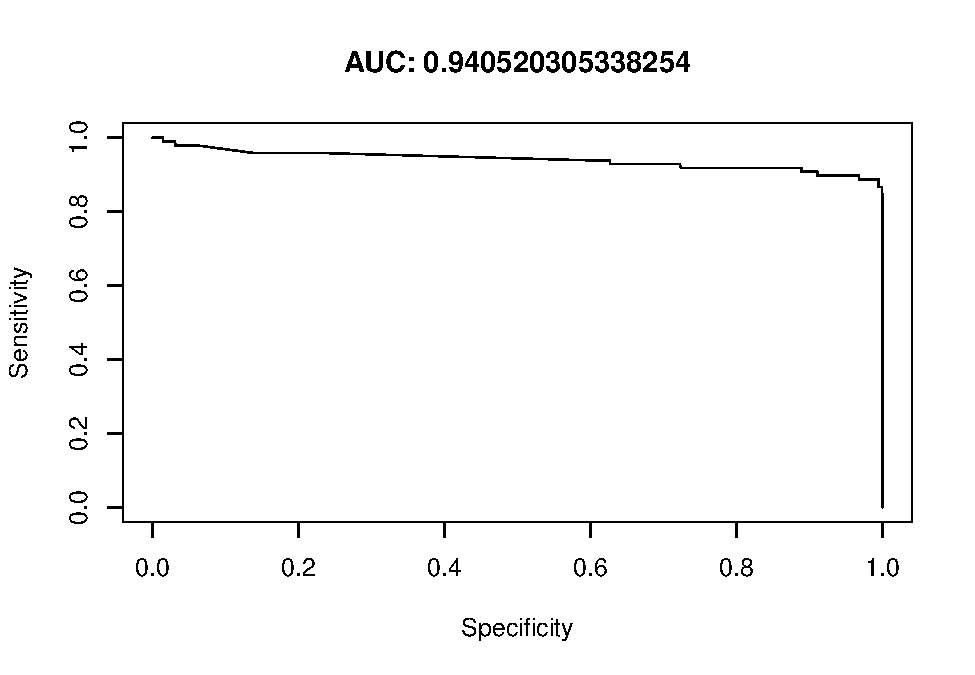
\includegraphics{Credit_Card_Fraud_Detection_Project_Report_files/figure-latex/unnamed-chunk-23-2} \end{center}

\begin{center}\includegraphics{Credit_Card_Fraud_Detection_Project_Report_files/figure-latex/unnamed-chunk-23-3} \end{center}

\begin{table}[H]
\centering\begingroup\fontsize{10}{12}\selectfont

\begin{tabular}{l|r|r}
\hline
Model & AUC & AUCPR\\
\hline
Naive Baseline - Predict Always Legal & 0.5000000 & 0.0000000\\
\hline
Naive Bayes & 0.9175977 & 0.0548969\\
\hline
K-Nearest Neighbors k=5 & 0.8162738 & 0.5797557\\
\hline
SVM - Support Vector Machine & 0.7751585 & 0.3196189\\
\hline
Random Forest & 0.8979328 & 0.7683457\\
\hline
GBM - Generalized Boosted Regression & 0.9538573 & 0.8421135\\
\hline
XGBoost & 0.9770390 & 0.8618163\\
\hline
LightGBM & 0.9405203 & 0.8545904\\
\hline
\end{tabular}
\endgroup{}
\end{table}

\begin{table}[H]
\centering\begingroup\fontsize{10}{12}\selectfont

\begin{tabular}{l|r|r|r}
\hline
Feature & Gain & Cover & Frequency\\
\hline
V14 & 0.4307962 & 0.3609848 & 0.0904762\\
\hline
V7 & 0.3035386 & 0.0323388 & 0.0304348\\
\hline
V12 & 0.0348256 & 0.0182142 & 0.0577640\\
\hline
V26 & 0.0338785 & 0.0063473 & 0.0654244\\
\hline
V10 & 0.0248953 & 0.0058810 & 0.0414079\\
\hline
V4 & 0.0243032 & 0.2500562 & 0.0921325\\
\hline
V20 & 0.0182291 & 0.0506729 & 0.0399586\\
\hline
V1 & 0.0093899 & 0.0008671 & 0.0252588\\
\hline
V18 & 0.0091918 & 0.0018870 & 0.0320911\\
\hline
V2 & 0.0086183 & 0.0015763 & 0.0225673\\
\hline
V16 & 0.0084501 & 0.0038963 & 0.0236025\\
\hline
V13 & 0.0082319 & 0.0032468 & 0.0322981\\
\hline
Amount & 0.0071959 & 0.0159475 & 0.0465839\\
\hline
V17 & 0.0068772 & 0.0408338 & 0.0225673\\
\hline
V28 & 0.0068020 & 0.0016715 & 0.0337474\\
\hline
V24 & 0.0062211 & 0.0023892 & 0.0293996\\
\hline
V15 & 0.0061126 & 0.0019022 & 0.0289855\\
\hline
V11 & 0.0050963 & 0.0335001 & 0.0260870\\
\hline
V6 & 0.0048581 & 0.0029185 & 0.0188406\\
\hline
V9 & 0.0048414 & 0.0010716 & 0.0287785\\
\hline
V3 & 0.0048409 & 0.0020941 & 0.0273292\\
\hline
V8 & 0.0047966 & 0.0138567 & 0.0207039\\
\hline
V27 & 0.0047570 & 0.0344483 & 0.0395445\\
\hline
V23 & 0.0046562 & 0.0377007 & 0.0333333\\
\hline
V25 & 0.0046264 & 0.0002474 & 0.0113872\\
\hline
V19 & 0.0043399 & 0.0126660 & 0.0182195\\
\hline
V22 & 0.0037440 & 0.0587793 & 0.0213251\\
\hline
V5 & 0.0032005 & 0.0024771 & 0.0229814\\
\hline
V21 & 0.0026854 & 0.0015272 & 0.0167702\\
\hline
\end{tabular}
\endgroup{}
\end{table}
\newpage

\hypertarget{results}{%
\section{Results}\label{results}}

This is the summary results for all the models builted, trained and
validated.

\begin{table}[H]
\centering\begingroup\fontsize{10}{12}\selectfont

\begin{tabular}{l|r|r}
\hline
Model & AUC & AUCPR\\
\hline
Naive Baseline - Predict Always Legal & 0.5000000 & 0.0000000\\
\hline
Naive Bayes & 0.9175977 & 0.0548969\\
\hline
K-Nearest Neighbors k=5 & 0.8162738 & 0.5797557\\
\hline
SVM - Support Vector Machine & 0.7751585 & 0.3196189\\
\hline
Random Forest & 0.8979328 & 0.7683457\\
\hline
GBM - Generalized Boosted Regression & 0.9538573 & 0.8421135\\
\hline
XGBoost & 0.9770390 & 0.8618163\\
\hline
LightGBM & 0.9405203 & 0.8545904\\
\hline
\end{tabular}
\endgroup{}
\end{table}

\hypertarget{conclusion}{%
\section{Conclusion}\label{conclusion}}

The ensemble methods once again confirm themselves as among the best
models out there. It easy to find them as a winners of numerous Kaggle's
competitions or on TOP5 of them. In this task, a XGBoost model can
achieve a very good AUCPR result of \textbf{0.86} and the others ensembe
methods are very close to it. As the features importance plots and table
show, there are few predictors like \textbf{V17} and \textbf{V14} that
are particularly useful for classifying a fraud. The SMOTE technique (a
technique for dealing with imbalanced data) could improve the
performance a little bit.

\newpage

\hypertarget{appendix}{%
\section{Appendix}\label{appendix}}

\hypertarget{a---all-visualization}{%
\subsection{1a - All visualization}\label{a---all-visualization}}

\begin{center}\includegraphics{Credit_Card_Fraud_Detection_Project_Report_files/figure-latex/unnamed-chunk-25-1} \end{center}

\begin{center}\includegraphics{Credit_Card_Fraud_Detection_Project_Report_files/figure-latex/unnamed-chunk-25-2} \end{center}

\begin{center}\includegraphics{Credit_Card_Fraud_Detection_Project_Report_files/figure-latex/unnamed-chunk-25-3} \end{center}

\begin{center}\includegraphics{Credit_Card_Fraud_Detection_Project_Report_files/figure-latex/unnamed-chunk-25-4} \end{center}

\begin{center}\includegraphics{Credit_Card_Fraud_Detection_Project_Report_files/figure-latex/unnamed-chunk-25-5} \end{center}

\begin{center}\includegraphics{Credit_Card_Fraud_Detection_Project_Report_files/figure-latex/unnamed-chunk-25-6} \end{center}

\begin{center}\includegraphics{Credit_Card_Fraud_Detection_Project_Report_files/figure-latex/unnamed-chunk-25-7} \end{center}

\begin{center}\includegraphics{Credit_Card_Fraud_Detection_Project_Report_files/figure-latex/unnamed-chunk-25-8} \end{center}

\begin{center}\includegraphics{Credit_Card_Fraud_Detection_Project_Report_files/figure-latex/unnamed-chunk-25-9} \end{center}

\begin{center}\includegraphics{Credit_Card_Fraud_Detection_Project_Report_files/figure-latex/unnamed-chunk-25-10} \end{center}

\begin{center}\includegraphics{Credit_Card_Fraud_Detection_Project_Report_files/figure-latex/unnamed-chunk-25-11} \end{center}

\begin{center}\includegraphics{Credit_Card_Fraud_Detection_Project_Report_files/figure-latex/unnamed-chunk-25-12} \end{center}

\begin{center}\includegraphics{Credit_Card_Fraud_Detection_Project_Report_files/figure-latex/unnamed-chunk-25-13} \end{center}

\begin{center}\includegraphics{Credit_Card_Fraud_Detection_Project_Report_files/figure-latex/unnamed-chunk-25-14} \end{center}

\begin{center}\includegraphics{Credit_Card_Fraud_Detection_Project_Report_files/figure-latex/unnamed-chunk-25-15} \end{center}

\begin{center}\includegraphics{Credit_Card_Fraud_Detection_Project_Report_files/figure-latex/unnamed-chunk-25-16} \end{center}

\begin{center}\includegraphics{Credit_Card_Fraud_Detection_Project_Report_files/figure-latex/unnamed-chunk-25-17} \end{center}

\begin{center}\includegraphics{Credit_Card_Fraud_Detection_Project_Report_files/figure-latex/unnamed-chunk-25-18} \end{center}

\begin{center}\includegraphics{Credit_Card_Fraud_Detection_Project_Report_files/figure-latex/unnamed-chunk-25-19} \end{center}

\begin{center}\includegraphics{Credit_Card_Fraud_Detection_Project_Report_files/figure-latex/unnamed-chunk-25-20} \end{center}

\begin{center}\includegraphics{Credit_Card_Fraud_Detection_Project_Report_files/figure-latex/unnamed-chunk-25-21} \end{center}

\begin{center}\includegraphics{Credit_Card_Fraud_Detection_Project_Report_files/figure-latex/unnamed-chunk-25-22} \end{center}

\begin{center}\includegraphics{Credit_Card_Fraud_Detection_Project_Report_files/figure-latex/unnamed-chunk-25-23} \end{center}

\begin{center}\includegraphics{Credit_Card_Fraud_Detection_Project_Report_files/figure-latex/unnamed-chunk-25-24} \end{center}

\begin{center}\includegraphics{Credit_Card_Fraud_Detection_Project_Report_files/figure-latex/unnamed-chunk-25-25} \end{center}

\begin{center}\includegraphics{Credit_Card_Fraud_Detection_Project_Report_files/figure-latex/unnamed-chunk-25-26} \end{center}

\hypertarget{b---code-used-in-this-report---credit-card-fraud-detection-project---code.r}{%
\subsection{1b - Code used in this report - Credit Card Fraud Detection
Project -
Code.R}\label{b---code-used-in-this-report---credit-card-fraud-detection-project---code.r}}

\begin{verbatim}
# Install all needed libraries if it is not present

if(!require(tidyverse)) install.packages("tidyverse") 
if(!require(kableExtra)) install.packages("kableExtra")
if(!require(tidyr)) install.packages("tidyr")
if(!require(tidyverse)) install.packages("tidyverse")
if(!require(stringr)) install.packages("stringr")
if(!require(ggplot2)) install.packages("ggplot2")
if(!require(gbm)) install.packages("gbm")
if(!require(dplyr)) install.packages("dplyr")
if(!require(caret)) install.packages("caret")
if(!require(xgboost)) install.packages("xgboost")
if(!require(e1071)) install.packages("e1071")
if(!require(class)) install.packages("class")
if(!require(ROCR)) install.packages("ROCR")
if(!require(randomForest)) install.packages("randomForest")
if(!require(PRROC)) install.packages("PRROC")
if(!require(reshape2)) install.packages("reshape2")

# Loading all needed libraries

library(dplyr)
library(tidyverse)
library(kableExtra)
library(tidyr)
library(ggplot2)
library(gbm)
library(caret)
library(xgboost)
library(e1071)
library(class)
library(lightgbm)
library(ROCR)
library(randomForest)
library(PRROC)
library(reshape2)

## Loading the dataset

creditcard <- read.csv("creditcard.csv")

# Check dimensions

data.frame("Length" = nrow(creditcard), "Columns" = ncol(creditcard)) %>%
kable() %>%
   kable_styling(bootstrap_options = c("striped", "hover", "condensed", "responsive"),
                 position = "center",
                 font_size = 10,
                 full_width = FALSE)
                 
imbalanced <- data.frame(creditcard)

imbalanced$Class = ifelse(creditcard$Class == 0, 'Legal', 'Fraud') %>% as.factor()

# Visualize the proportion between classes

imbalanced %>%
  ggplot(aes(Class)) +
  theme_minimal()  +
  geom_bar() +
  scale_x_discrete() +
  scale_y_continuous(labels = scales::comma) +
  labs(title = "Proportions between Legal and Frauds Transactions",
        x = "Class",
        y = "Frequency")
        
# Find missing values

sapply(creditcard, function(x) sum(is.na(x))) %>% 
kable(col.names = c("Missing Values")) %>%
   kable_styling(bootstrap_options = c("striped", "hover", "condensed", "responsive"),
                 position = "center",
                 font_size = 10,
                 full_width = FALSE)
                 
# Frauds Amount

creditcard[creditcard$Class == 1,] %>%
  ggplot(aes(Amount)) + 
  theme_minimal()  +
  geom_histogram(binwidth = 40) +
  labs(title = "Frauds Amounts Distributions",
        x = "Amount in dollars",
        y = "Frequency")

creditcard[creditcard$Class == 1,] %>%
  group_by(Amount) %>%
  summarise(count = n()) %>%
  arrange(desc(count)) %>%
  head(n=10) %>%
  kable() %>%
  kable_styling(bootstrap_options = c("striped", "hover", "condensed", "responsive"),
                 position = "center",
                 font_size = 10,
                 full_width = FALSE)
                 
# Frauds over Time

creditcard[creditcard$Class == 1,] %>%
  ggplot(aes(Time)) + 
  theme_minimal()  +
  geom_histogram(binwidth = 40) +
  labs(title = "Frauds over Time Distributions",
        x = "Time",
        y = "Frequency")

creditcard[creditcard$Class == 1,] %>%
  group_by(Time) %>%
  summarise(count = n()) %>%
  arrange(desc(count)) %>%
  head(n=10) %>%
  kable() %>%
  kable_styling(bootstrap_options = c("striped", "hover", "condensed", "responsive"),
                 position = "center",
                 font_size = 10,
                 full_width = FALSE)

# Get lower triangle of the correlation matrix

get_lower_tri<-function(cormat){
  cormat[upper.tri(cormat)] <- NA
  return(cormat)
}

# Get upper triangle of the correlation matrix

get_upper_tri <- function(cormat){
  cormat[lower.tri(cormat)]<- NA
  return(cormat)
}

reorder_cormat <- function(cormat){
  # Use correlation between variables as distance
  dd <- as.dist((1-cormat)/2)
  hc <- hclust(dd)
  cormat <-cormat[hc$order, hc$order]
}

corr_matrix <- round(cor(creditcard),2)
corr_matrix <- reorder_cormat(corr_matrix)

upper_tri <- get_upper_tri(corr_matrix)

melted_corr_matrix <- melt(upper_tri, na.rm = TRUE)

ggplot(melted_corr_matrix, aes(Var2, Var1, fill = value)) +
geom_tile(color = "white") +
scale_fill_gradient2(low = "blue", high = "red", mid = "white", 
   midpoint = 0, limit = c(-1,1), space = "Lab", 
   name="Pearson\nCorrelation") +
   theme_minimal() + 
   theme(axis.text.x = element_text(angle = 90, vjust = 1, 
         size = 9, hjust = 1), axis.text.y = element_text(size = 9),                    axis.title.x = element_blank(),
         axis.title.y = element_blank(),
         panel.grid.major = element_blank(),
         panel.border = element_blank(),
         panel.background = element_blank(),
         axis.ticks = element_blank()) +
 coord_fixed()
 
# Set seed for reproducibility

set.seed(1234)

# Remove the "Time" column from the dataset

creditcard$Class <- as.factor(creditcard$Class)
creditcard <- creditcard %>% select(-Time)

# Split the dataset into train, test dataset and cv

train_index <- createDataPartition(
  y = creditcard$Class, 
  p = .6, 
  list = F
)

train <- creditcard[train_index,]

test_cv <- creditcard[-train_index,]

test_index <- createDataPartition(
  y = test_cv$Class, 
  p = .5, 
  list = F)

test <- test_cv[test_index,]
cv <- test_cv[-test_index,]

rm(train_index, test_index, test_cv)
 
# Create a baseline model that predict always "legal" 
# (aka "0") transactions and compute all metrics

# Clone the creditcard dataframe

baseline_model <- data.frame(creditcard)

# Set Class al to Legal (0)

baseline_model$Class = factor(0, c(0,1))

# Make predictions

pred <- prediction(
  as.numeric(as.character(baseline_model$Class)),                        as.numeric(as.character(creditcard$Class))
)

# Compute the AUC and AUCPR

auc_val_baseline <- performance(pred, "auc")
auc_plot_baseline <- performance(pred, 'sens', 'spec')
aucpr_plot_baseline <- performance(pred, "prec", "rec")

# Make the relative plot

plot(auc_plot_baseline, 
     main=paste("AUC:", 
     auc_val_baseline@y.values[[1]])
)

plot(aucpr_plot_baseline, main="AUCPR: 0")

# Create a dataframe 'results' that contains all metrics 
# obtained by the trained models

results <- data.frame(
  Model = "Naive Baseline - Predict Always Legal", 
  AUC = auc_val_baseline@y.values[[1]],
  AUCPR = 0
)

# Show results on a table

results %>% 
  kable() %>%
  kable_styling(
    bootstrap_options = 
      c("striped", "hover", "condensed", "responsive"),
      position = "center",
      font_size = 10,
      full_width = FALSE
) 
 
# Create a Naive Bayes Model, it will improve a little bit the 
# results in AUC and AUCPR

# Set seed 1234 for reproducibility

set.seed(1234)

# Build the model with Class as target and all other variables
# as predictors

naive_model <- naiveBayes(Class ~ ., data = train, laplace=1)

# Predict

predictions <- predict(naive_model, newdata=test)

# Compute the AUC and AUCPR for the Naive Model

pred <- prediction(as.numeric(predictions) , test$Class)

auc_val_naive <- performance(pred, "auc")

auc_plot_naive <- performance(pred, 'sens', 'spec')
aucpr_plot_naive <- performance(pred, "prec", "rec")

aucpr_val_naive <- pr.curve(
  scores.class0 = predictions[test$Class == 1], 
  scores.class1 = predictions[test$Class == 0],
  curve = T,  
  dg.compute = T
)

# Make the relative plot

plot(aucpr_val_naive)
plot(auc_plot_naive, main=paste("AUC:", auc_val_naive@y.values[[1]]))
plot(aucpr_plot_naive, main=paste("AUCPR:", aucpr_val_naive$auc.integral))

# Adding the respective metrics to the results dataset

results <- results %>% add_row(
  Model = "Naive Bayes", 
  AUC = auc_val_naive@y.values[[1]],
  AUCPR = aucpr_val_naive$auc.integral
)

# Show results on a table

results %>%
  kable() %>%
  kable_styling(bootstrap_options = c("striped", "hover", "condensed",           "responsive"),
      position = "center",
      font_size = 10,
      full_width = FALSE) 
 
# Set seed 1234 for reproducibility

set.seed(1234)

# Build a KNN Model with Class as Target and all other
# variables as predictors. k is set to 5

knn_model <- knn(train[,-30], test[,-30], train$Class, k=5, prob = TRUE)

# Compute the AUC and AUCPR for the KNN Model

pred <- prediction(
  as.numeric(as.character(knn_model)),                                   as.numeric(as.character(test$Class))
)

auc_val_knn <- performance(pred, "auc")

auc_plot_knn <- performance(pred, 'sens', 'spec')
aucpr_plot_knn <- performance(pred, "prec", "rec")

aucpr_val_knn <- pr.curve(
  scores.class0 = knn_model[test$Class == 1], 
  scores.class1 = knn_model[test$Class == 0],
  curve = T,  
  dg.compute = T
)

# Make the relative plot

plot(aucpr_val_knn)
plot(auc_plot_knn, main=paste("AUC:", auc_val_knn@y.values[[1]]))
plot(aucpr_plot_knn, main=paste("AUCPR:", aucpr_val_knn$auc.integral))

# Adding the respective metrics to the results dataset

results <- results %>% add_row(
  Model = "K-Nearest Neighbors k=5", 
  AUC = auc_val_knn@y.values[[1]],
  AUCPR = aucpr_val_knn$auc.integral
)

# Show results on a table

results %>%
   kable() %>%
   kable_styling(bootstrap_options = c("striped", "hover", "condensed",           "responsive"),
       position = "center",
       font_size = 10,
       full_width = FALSE) 
 
# Set seed 1234 for reproducibility

set.seed(1234)

# Build a SVM Model with Class as Target and all other
# variables as predictors. The kernel is set to sigmoid

svm_model <- svm(Class ~ ., data = train, kernel='sigmoid')

# Make predictions based on this model

predictions <- predict(svm_model, newdata=test)

# Compute AUC and AUCPR

pred <- prediction(
  as.numeric(as.character(predictions)),                                 as.numeric(as.character(test$Class))
)

auc_val_svm <- performance(pred, "auc")

auc_plot_svm <- performance(pred, 'sens', 'spec')
aucpr_plot_svm <- performance(pred, "prec", "rec")

aucpr_val_svm <- pr.curve(
  scores.class0 = predictions[test$Class == 1], 
  scores.class1 = predictions[test$Class == 0],
  curve = T,  
  dg.compute = T
)

# Make the relative plot

plot(aucpr_val_svm)
plot(auc_plot_svm, main=paste("AUC:", auc_val_svm@y.values[[1]]))
plot(aucpr_plot_svm, main=paste("AUCPR:", aucpr_val_svm$auc.integral))

# Adding the respective metrics to the results dataset

results <- results %>% add_row(
  Model = "SVM - Support Vector Machine",
  AUC = auc_val_svm@y.values[[1]],
  AUCPR = aucpr_val_svm$auc.integral)

# Show results on a table

results %>%
  kable() %>%
  kable_styling(bootstrap_options = c("striped", "hover", "condensed",           "responsive"),
      position = "center",
      font_size = 10,
      full_width = FALSE)
 
# Set seed 1234 for reproducibility

set.seed(1234)

# Build a Random Forest Model with Class as Target and all other
# variables as predictors. The number of trees is set to 500

rf_model <- randomForest(Class ~ ., data = train, ntree = 500)

# Get the feature importance

feature_imp_rf <- data.frame(importance(rf_model))

# Make predictions based on this model

predictions <- predict(rf_model, newdata=test)

# Compute the AUC and AUPCR

pred <- prediction(
  as.numeric(as.character(predictions)),                                 as.numeric(as.character(test$Class))
)

auc_val_rf <- performance(pred, "auc")

auc_plot_rf <- performance(pred, 'sens', 'spec')

aucpr_plot_rf <- performance(pred, "prec", "rec", curve = T,  dg.compute = T)

aucpr_val_rf <- pr.curve(scores.class0 = predictions[test$Class == 1], scores.class1 = predictions[test$Class == 0],curve = T,  dg.compute = T)

# make the relative plot

plot(auc_plot_rf, main=paste("AUC:", auc_val_rf@y.values[[1]]))
plot(aucpr_plot_rf, main=paste("AUCPR:", aucpr_val_rf$auc.integral))
plot(aucpr_val_rf)

# Adding the respective metrics to the results dataset

results <- results %>% add_row(
  Model = "Random Forest",
  AUC = auc_val_rf@y.values[[1]],
  AUCPR = aucpr_val_rf$auc.integral)

# Show results on a table

results %>%
  kable() %>%
  kable_styling(bootstrap_options = c("striped", "hover", "condensed",           "responsive"),
      position = "center",
      font_size = 10,
      full_width = FALSE)

# Show feature importance on a table

feature_imp_rf %>%
  kable() %>%
  kable_styling(bootstrap_options = c("striped", "hover", "condensed",           "responsive"),
      position = "center",
      font_size = 10,
      full_width = FALSE)
 
# Set seet 1234 for reproducibility

set.seed(1234)

# Build a GBM Model with Class as Target and all other
# variables as predictors. Distribution is bernoully, 
# number of tree is 500

gbm_model <- gbm(as.character(Class) ~ .,
                 distribution = "bernoulli", 
                 data = rbind(train, test), 
                 n.trees = 500,
                 interaction.depth = 3, 
                 n.minobsinnode = 100, 
                 shrinkage = 0.01, 
                 train.fraction = 0.7,
)

# Determine the best iteration based on test data

best_iter = gbm.perf(gbm_model, method = "test")

# Make predictions based on this model

predictions = predict.gbm(
  gbm_model, 
  newdata = test, 
  n.trees = best_iter, 
  type="response"
)

# Get feature importance

feature_imp_gbm = summary(gbm_model, n.trees = best_iter)

# Compute the AUC and AUPCR

pred <- prediction(
  as.numeric(as.character(predictions)),                                 as.numeric(as.character(test$Class))
)

auc_val_gbm <- performance(pred, "auc")

auc_plot_gbm <- performance(pred, 'sens', 'spec')
aucpr_plot_gbm <- performance(pred, "prec", "rec")

aucpr_val_gbm <- pr.curve(
  scores.class0 = predictions[test$Class == 1], 
  scores.class1 = predictions[test$Class == 0],
  curve = T,  
  dg.compute = T
)

# Make the relative plot

plot(aucpr_val_gbm)
plot(auc_plot_gbm, main=paste("AUC:", auc_val_gbm@y.values[[1]]))
plot(aucpr_plot_gbm, main=paste("AUCPR:", aucpr_val_gbm$auc.integral))

# Adding the respective metrics to the results dataset

results <- results %>% add_row(
  Model = "GBM - Generalized Boosted Regression",
  AUC = auc_val_gbm@y.values[[1]],
  AUCPR = aucpr_val_gbm$auc.integral)

# Show results on a table

results %>%
  kable() %>%
  kable_styling(bootstrap_options = c("striped", "hover", "condensed",           "responsive"),
      position = "center",
      font_size = 10,
      full_width = FALSE)

# Show feature importance on a table

feature_imp_gbm %>%
  kable() %>%
  kable_styling(bootstrap_options = c("striped", "hover", "condensed",           "responsive"),
      position = "center",
      font_size = 10,
      full_width = FALSE) 
 
# Set seet 1234 for reproducibility

set.seed(1234)

# Prepare the training dataset

xgb_train <- xgb.DMatrix(
  as.matrix(train[, colnames(train) != "Class"]), 
  label = as.numeric(as.character(train$Class))
)

# Prepare the test dataset

xgb_test <- xgb.DMatrix(
  as.matrix(test[, colnames(test) != "Class"]), 
  label = as.numeric(as.character(test$Class))
)

# Prepare the cv dataset

xgb_cv <- xgb.DMatrix(
  as.matrix(cv[, colnames(cv) != "Class"]), 
  label = as.numeric(as.character(cv$Class))
)

# Prepare the parameters list. 

xgb_params <- list(
  objective = "binary:logistic", 
  eta = 0.1, 
  max.depth = 3, 
  nthread = 6, 
  eval_metric = "aucpr"
)

# Train the XGBoost Model

xgb_model <- xgb.train(
  data = xgb_train, 
  params = xgb_params, 
  watchlist = list(test = xgb_test, cv = xgb_cv), 
  nrounds = 500, 
  early_stopping_rounds = 40, 
  print_every_n = 20
)

# Get feature importance

feature_imp_xgb <- xgb.importance(colnames(train), model = xgb_model)

xgb.plot.importance(feature_imp_xgb, rel_to_first = TRUE, xlab = "Relative importance")

# Make predictions based on this model

predictions = predict(
  xgb_model, 
  newdata = as.matrix(test[, colnames(test) != "Class"]), 
  ntreelimit = xgb_model$bestInd
)

# Compute the AUC and AUPCR

pred <- prediction(
  as.numeric(as.character(predictions)),                                 as.numeric(as.character(test$Class))
)

auc_val_xgb <- performance(pred, "auc")

auc_plot_xgb <- performance(pred, 'sens', 'spec')
aucpr_plot_xgb <- performance(pred, "prec", "rec")

aucpr_val_xgb <- pr.curve(
  scores.class0 = predictions[test$Class == 1], 
  scores.class1 = predictions[test$Class == 0],
  curve = T,  
  dg.compute = T
)

# Make the relative plot

plot(auc_plot_xgb, main=paste("AUC:", auc_val_xgb@y.values[[1]]))
plot(aucpr_plot_xgb, main=paste("AUCPR:", aucpr_val_xgb$auc.integral))
plot(aucpr_val_xgb)

# Adding the respective metrics to the results dataset

results <- results %>% add_row(
  Model = "XGBoost",
  AUC = auc_val_xgb@y.values[[1]],
  AUCPR = aucpr_val_xgb$auc.integral)

# Show results on a table

results %>%
  kable() %>%
  kable_styling(bootstrap_options = c("striped", "hover", "condensed",           "responsive"),
      position = "center",
      font_size = 10,
      full_width = FALSE)

# Show feature importance on a table

feature_imp_xgb %>%
  kable() %>%
  kable_styling(bootstrap_options = c("striped", "hover", "condensed",           "responsive"),
      position = "center",
      font_size = 10,
      full_width = FALSE)
      
# Set seet 1234 for reproducibility

set.seed(1234)

# Prepare the training dataset

lgb_train <- lgb.Dataset(
  as.matrix(train[, colnames(train) != "Class"]), 
  label = as.numeric(as.character(train$Class))
)

# Prepare the test dataset

lgb_test <- lgb.Dataset(
  as.matrix(test[, colnames(test) != "Class"]), 
  label = as.numeric(as.character(test$Class))
)

# Prepare the cvtaset

lgb_cv <- lgb.Dataset(
  as.matrix(cv[, colnames(cv) != "Class"]), 
  label = as.numeric(as.character(cv$Class))
)

# Prepare the parameters list

lgb_params = list(
    objective = "binary", 
    metric = "binary_error"
)

# Train the LightGBM Model

lgb_model <- lgb.train(
        params = lgb_params, 
        data = lgb_train, 
        valids = list(test = lgb_test, cv = lgb_cv), 
        learning_rate = 0.01, 
        nrounds = 500,
        early_stopping_rounds = 40, 
        eval_freq = 20
)

# Get feature importance

feature_imp_lgb = lgb.importance(lgb_model, percentage = TRUE)

# Make predictions based on this model

predictions = predict(
  lgb_model, 
  data = as.matrix(test[, colnames(test) != "Class"]), 
  n = lgb_model$best_iter)

# Compute the AUC and AUPCR

pred <- prediction(
  predictions, 
  as.numeric(as.character(test$Class))
)

auc_val_lgb <- performance(pred, "auc")

auc_plot_lgb <- performance(pred, 'sens', 'spec')
aucpr_plot_lgb <- performance(pred, "prec", "rec")

aucpr_val_lgb <- pr.curve(
  scores.class0 = predictions[test$Class == 1], 
  scores.class1 = predictions[test$Class == 0],
  curve = T,  
  dg.compute = T
)

# Make the relative plot

plot(aucpr_val_lgb)
plot(auc_plot_lgb, main=paste("AUC:", auc_val_lgb@y.values[[1]]))
plot(aucpr_plot_lgb, main=paste("AUCPR:", aucpr_val_lgb$auc.integral))

# Adding the respective metrics to the results dataset

results <- results %>% add_row(
  Model = "LightGBM",
  AUC = auc_val_lgb@y.values[[1]],
  AUCPR = aucpr_val_lgb$auc.integral
  )

# Show results on a table

results %>%
  kable() %>%
  kable_styling(bootstrap_options = c("striped", "hover", "condensed",           "responsive"),
      position = "center",
      font_size = 10,
      full_width = FALSE)

feature_imp_lgb %>%
  kable() %>%
  kable_styling(bootstrap_options = c("striped", "hover", "condensed",           "responsive"),
      position = "center",
      font_size = 10,
      full_width = FALSE)
\end{verbatim}

\hypertarget{c---enviroment}{%
\subsection{1c - Enviroment}\label{c---enviroment}}

\begin{verbatim}
## [1] "Operating System:"
\end{verbatim}

\begin{verbatim}
##                _                           
## platform       x86_64-w64-mingw32          
## arch           x86_64                      
## os             mingw32                     
## system         x86_64, mingw32             
## status                                     
## major          3                           
## minor          6.0                         
## year           2019                        
## month          04                          
## day            26                          
## svn rev        76424                       
## language       R                           
## version.string R version 3.6.0 (2019-04-26)
## nickname       Planting of a Tree
\end{verbatim}

\begin{verbatim}
## [1] "All installed packages"
\end{verbatim}

\begin{verbatim}
##               Package        
## abind         "abind"        
## askpass       "askpass"      
## assertthat    "assertthat"   
## backports     "backports"    
## base64enc     "base64enc"    
## BH            "BH"           
## bitops        "bitops"       
## broom         "broom"        
## callr         "callr"        
## caret         "caret"        
## caTools       "caTools"      
## cellranger    "cellranger"   
## Ckmeans.1d.dp "Ckmeans.1d.dp"
## class         "class"        
## cli           "cli"          
## clipr         "clipr"        
## colorspace    "colorspace"   
## crayon        "crayon"       
## curl          "curl"         
## data.table    "data.table"   
## DBI           "DBI"          
## dbplyr        "dbplyr"       
## digest        "digest"       
## DMwR          "DMwR"         
## DMwR2         "DMwR2"        
## doParallel    "doParallel"   
## dplyr         "dplyr"        
## dslabs        "dslabs"       
## e1071         "e1071"        
## ellipsis      "ellipsis"     
## evaluate      "evaluate"     
## fansi         "fansi"        
## forcats       "forcats"      
## foreach       "foreach"      
## fs            "fs"           
## gbm           "gbm"          
## gdata         "gdata"        
## generics      "generics"     
## ggplot2       "ggplot2"      
## glue          "glue"         
## gower         "gower"        
## gplots        "gplots"       
## gridExtra     "gridExtra"    
## gtable        "gtable"       
## gtools        "gtools"       
## haven         "haven"        
## highr         "highr"        
## hms           "hms"          
## htmltools     "htmltools"    
## httr          "httr"         
## ipred         "ipred"        
## iterators     "iterators"    
## jsonlite      "jsonlite"     
## kableExtra    "kableExtra"   
## knitr         "knitr"        
## labeling      "labeling"     
## lattice       "lattice"      
## lava          "lava"         
## lazyeval      "lazyeval"     
## lightgbm      "lightgbm"     
## lubridate     "lubridate"    
## magrittr      "magrittr"     
## markdown      "markdown"     
## mime          "mime"         
## ModelMetrics  "ModelMetrics" 
## modelr        "modelr"       
## munsell       "munsell"      
## numDeriv      "numDeriv"     
## openssl       "openssl"      
## PerfMeas      "PerfMeas"     
## pillar        "pillar"       
## pkgconfig     "pkgconfig"    
## plogr         "plogr"        
## plyr          "plyr"         
## precrec       "precrec"      
## prettyunits   "prettyunits"  
## pROC          "pROC"         
## processx      "processx"     
## prodlim       "prodlim"      
## progress      "progress"     
## PRROC         "PRROC"        
## ps            "ps"           
## purrr         "purrr"        
## quantmod      "quantmod"     
## R6            "R6"           
## randomForest  "randomForest" 
## RColorBrewer  "RColorBrewer" 
## Rcpp          "Rcpp"         
## RcppRoll      "RcppRoll"     
## readr         "readr"        
## readxl        "readxl"       
## recipes       "recipes"      
## rematch       "rematch"      
## reprex        "reprex"       
## reshape2      "reshape2"     
## rlang         "rlang"        
## rmarkdown     "rmarkdown"    
## ROCR          "ROCR"         
## rprojroot     "rprojroot"    
## rstudioapi    "rstudioapi"   
## rvest         "rvest"        
## scales        "scales"       
## selectr       "selectr"      
## SQUAREM       "SQUAREM"      
## stringi       "stringi"      
## stringr       "stringr"      
## sys           "sys"          
## tibble        "tibble"       
## tidyr         "tidyr"        
## tidyselect    "tidyselect"   
## tidyverse     "tidyverse"    
## timeDate      "timeDate"     
## tinytex       "tinytex"      
## TTR           "TTR"          
## utf8          "utf8"         
## vctrs         "vctrs"        
## viridisLite   "viridisLite"  
## webshot       "webshot"      
## whisker       "whisker"      
## withr         "withr"        
## xfun          "xfun"         
## xgboost       "xgboost"      
## xml2          "xml2"         
## xts           "xts"          
## yaml          "yaml"         
## zeallot       "zeallot"      
## zoo           "zoo"          
## base          "base"         
## boot          "boot"         
## class         "class"        
## cluster       "cluster"      
## codetools     "codetools"    
## compiler      "compiler"     
## datasets      "datasets"     
## foreign       "foreign"      
## graphics      "graphics"     
## grDevices     "grDevices"    
## grid          "grid"         
## KernSmooth    "KernSmooth"   
## lattice       "lattice"      
## MASS          "MASS"         
## Matrix        "Matrix"       
## methods       "methods"      
## mgcv          "mgcv"         
## nlme          "nlme"         
## nnet          "nnet"         
## parallel      "parallel"     
## rpart         "rpart"        
## spatial       "spatial"      
## splines       "splines"      
## stats         "stats"        
## stats4        "stats4"       
## survival      "survival"     
## tcltk         "tcltk"        
## tools         "tools"        
## translations  "translations" 
## utils         "utils"        
##               LibPath                                              
## abind         "C:/Users/aless/OneDrive/Documenti/R/win-library/3.6"
## askpass       "C:/Users/aless/OneDrive/Documenti/R/win-library/3.6"
## assertthat    "C:/Users/aless/OneDrive/Documenti/R/win-library/3.6"
## backports     "C:/Users/aless/OneDrive/Documenti/R/win-library/3.6"
## base64enc     "C:/Users/aless/OneDrive/Documenti/R/win-library/3.6"
## BH            "C:/Users/aless/OneDrive/Documenti/R/win-library/3.6"
## bitops        "C:/Users/aless/OneDrive/Documenti/R/win-library/3.6"
## broom         "C:/Users/aless/OneDrive/Documenti/R/win-library/3.6"
## callr         "C:/Users/aless/OneDrive/Documenti/R/win-library/3.6"
## caret         "C:/Users/aless/OneDrive/Documenti/R/win-library/3.6"
## caTools       "C:/Users/aless/OneDrive/Documenti/R/win-library/3.6"
## cellranger    "C:/Users/aless/OneDrive/Documenti/R/win-library/3.6"
## Ckmeans.1d.dp "C:/Users/aless/OneDrive/Documenti/R/win-library/3.6"
## class         "C:/Users/aless/OneDrive/Documenti/R/win-library/3.6"
## cli           "C:/Users/aless/OneDrive/Documenti/R/win-library/3.6"
## clipr         "C:/Users/aless/OneDrive/Documenti/R/win-library/3.6"
## colorspace    "C:/Users/aless/OneDrive/Documenti/R/win-library/3.6"
## crayon        "C:/Users/aless/OneDrive/Documenti/R/win-library/3.6"
## curl          "C:/Users/aless/OneDrive/Documenti/R/win-library/3.6"
## data.table    "C:/Users/aless/OneDrive/Documenti/R/win-library/3.6"
## DBI           "C:/Users/aless/OneDrive/Documenti/R/win-library/3.6"
## dbplyr        "C:/Users/aless/OneDrive/Documenti/R/win-library/3.6"
## digest        "C:/Users/aless/OneDrive/Documenti/R/win-library/3.6"
## DMwR          "C:/Users/aless/OneDrive/Documenti/R/win-library/3.6"
## DMwR2         "C:/Users/aless/OneDrive/Documenti/R/win-library/3.6"
## doParallel    "C:/Users/aless/OneDrive/Documenti/R/win-library/3.6"
## dplyr         "C:/Users/aless/OneDrive/Documenti/R/win-library/3.6"
## dslabs        "C:/Users/aless/OneDrive/Documenti/R/win-library/3.6"
## e1071         "C:/Users/aless/OneDrive/Documenti/R/win-library/3.6"
## ellipsis      "C:/Users/aless/OneDrive/Documenti/R/win-library/3.6"
## evaluate      "C:/Users/aless/OneDrive/Documenti/R/win-library/3.6"
## fansi         "C:/Users/aless/OneDrive/Documenti/R/win-library/3.6"
## forcats       "C:/Users/aless/OneDrive/Documenti/R/win-library/3.6"
## foreach       "C:/Users/aless/OneDrive/Documenti/R/win-library/3.6"
## fs            "C:/Users/aless/OneDrive/Documenti/R/win-library/3.6"
## gbm           "C:/Users/aless/OneDrive/Documenti/R/win-library/3.6"
## gdata         "C:/Users/aless/OneDrive/Documenti/R/win-library/3.6"
## generics      "C:/Users/aless/OneDrive/Documenti/R/win-library/3.6"
## ggplot2       "C:/Users/aless/OneDrive/Documenti/R/win-library/3.6"
## glue          "C:/Users/aless/OneDrive/Documenti/R/win-library/3.6"
## gower         "C:/Users/aless/OneDrive/Documenti/R/win-library/3.6"
## gplots        "C:/Users/aless/OneDrive/Documenti/R/win-library/3.6"
## gridExtra     "C:/Users/aless/OneDrive/Documenti/R/win-library/3.6"
## gtable        "C:/Users/aless/OneDrive/Documenti/R/win-library/3.6"
## gtools        "C:/Users/aless/OneDrive/Documenti/R/win-library/3.6"
## haven         "C:/Users/aless/OneDrive/Documenti/R/win-library/3.6"
## highr         "C:/Users/aless/OneDrive/Documenti/R/win-library/3.6"
## hms           "C:/Users/aless/OneDrive/Documenti/R/win-library/3.6"
## htmltools     "C:/Users/aless/OneDrive/Documenti/R/win-library/3.6"
## httr          "C:/Users/aless/OneDrive/Documenti/R/win-library/3.6"
## ipred         "C:/Users/aless/OneDrive/Documenti/R/win-library/3.6"
## iterators     "C:/Users/aless/OneDrive/Documenti/R/win-library/3.6"
## jsonlite      "C:/Users/aless/OneDrive/Documenti/R/win-library/3.6"
## kableExtra    "C:/Users/aless/OneDrive/Documenti/R/win-library/3.6"
## knitr         "C:/Users/aless/OneDrive/Documenti/R/win-library/3.6"
## labeling      "C:/Users/aless/OneDrive/Documenti/R/win-library/3.6"
## lattice       "C:/Users/aless/OneDrive/Documenti/R/win-library/3.6"
## lava          "C:/Users/aless/OneDrive/Documenti/R/win-library/3.6"
## lazyeval      "C:/Users/aless/OneDrive/Documenti/R/win-library/3.6"
## lightgbm      "C:/Users/aless/OneDrive/Documenti/R/win-library/3.6"
## lubridate     "C:/Users/aless/OneDrive/Documenti/R/win-library/3.6"
## magrittr      "C:/Users/aless/OneDrive/Documenti/R/win-library/3.6"
## markdown      "C:/Users/aless/OneDrive/Documenti/R/win-library/3.6"
## mime          "C:/Users/aless/OneDrive/Documenti/R/win-library/3.6"
## ModelMetrics  "C:/Users/aless/OneDrive/Documenti/R/win-library/3.6"
## modelr        "C:/Users/aless/OneDrive/Documenti/R/win-library/3.6"
## munsell       "C:/Users/aless/OneDrive/Documenti/R/win-library/3.6"
## numDeriv      "C:/Users/aless/OneDrive/Documenti/R/win-library/3.6"
## openssl       "C:/Users/aless/OneDrive/Documenti/R/win-library/3.6"
## PerfMeas      "C:/Users/aless/OneDrive/Documenti/R/win-library/3.6"
## pillar        "C:/Users/aless/OneDrive/Documenti/R/win-library/3.6"
## pkgconfig     "C:/Users/aless/OneDrive/Documenti/R/win-library/3.6"
## plogr         "C:/Users/aless/OneDrive/Documenti/R/win-library/3.6"
## plyr          "C:/Users/aless/OneDrive/Documenti/R/win-library/3.6"
## precrec       "C:/Users/aless/OneDrive/Documenti/R/win-library/3.6"
## prettyunits   "C:/Users/aless/OneDrive/Documenti/R/win-library/3.6"
## pROC          "C:/Users/aless/OneDrive/Documenti/R/win-library/3.6"
## processx      "C:/Users/aless/OneDrive/Documenti/R/win-library/3.6"
## prodlim       "C:/Users/aless/OneDrive/Documenti/R/win-library/3.6"
## progress      "C:/Users/aless/OneDrive/Documenti/R/win-library/3.6"
## PRROC         "C:/Users/aless/OneDrive/Documenti/R/win-library/3.6"
## ps            "C:/Users/aless/OneDrive/Documenti/R/win-library/3.6"
## purrr         "C:/Users/aless/OneDrive/Documenti/R/win-library/3.6"
## quantmod      "C:/Users/aless/OneDrive/Documenti/R/win-library/3.6"
## R6            "C:/Users/aless/OneDrive/Documenti/R/win-library/3.6"
## randomForest  "C:/Users/aless/OneDrive/Documenti/R/win-library/3.6"
## RColorBrewer  "C:/Users/aless/OneDrive/Documenti/R/win-library/3.6"
## Rcpp          "C:/Users/aless/OneDrive/Documenti/R/win-library/3.6"
## RcppRoll      "C:/Users/aless/OneDrive/Documenti/R/win-library/3.6"
## readr         "C:/Users/aless/OneDrive/Documenti/R/win-library/3.6"
## readxl        "C:/Users/aless/OneDrive/Documenti/R/win-library/3.6"
## recipes       "C:/Users/aless/OneDrive/Documenti/R/win-library/3.6"
## rematch       "C:/Users/aless/OneDrive/Documenti/R/win-library/3.6"
## reprex        "C:/Users/aless/OneDrive/Documenti/R/win-library/3.6"
## reshape2      "C:/Users/aless/OneDrive/Documenti/R/win-library/3.6"
## rlang         "C:/Users/aless/OneDrive/Documenti/R/win-library/3.6"
## rmarkdown     "C:/Users/aless/OneDrive/Documenti/R/win-library/3.6"
## ROCR          "C:/Users/aless/OneDrive/Documenti/R/win-library/3.6"
## rprojroot     "C:/Users/aless/OneDrive/Documenti/R/win-library/3.6"
## rstudioapi    "C:/Users/aless/OneDrive/Documenti/R/win-library/3.6"
## rvest         "C:/Users/aless/OneDrive/Documenti/R/win-library/3.6"
## scales        "C:/Users/aless/OneDrive/Documenti/R/win-library/3.6"
## selectr       "C:/Users/aless/OneDrive/Documenti/R/win-library/3.6"
## SQUAREM       "C:/Users/aless/OneDrive/Documenti/R/win-library/3.6"
## stringi       "C:/Users/aless/OneDrive/Documenti/R/win-library/3.6"
## stringr       "C:/Users/aless/OneDrive/Documenti/R/win-library/3.6"
## sys           "C:/Users/aless/OneDrive/Documenti/R/win-library/3.6"
## tibble        "C:/Users/aless/OneDrive/Documenti/R/win-library/3.6"
## tidyr         "C:/Users/aless/OneDrive/Documenti/R/win-library/3.6"
## tidyselect    "C:/Users/aless/OneDrive/Documenti/R/win-library/3.6"
## tidyverse     "C:/Users/aless/OneDrive/Documenti/R/win-library/3.6"
## timeDate      "C:/Users/aless/OneDrive/Documenti/R/win-library/3.6"
## tinytex       "C:/Users/aless/OneDrive/Documenti/R/win-library/3.6"
## TTR           "C:/Users/aless/OneDrive/Documenti/R/win-library/3.6"
## utf8          "C:/Users/aless/OneDrive/Documenti/R/win-library/3.6"
## vctrs         "C:/Users/aless/OneDrive/Documenti/R/win-library/3.6"
## viridisLite   "C:/Users/aless/OneDrive/Documenti/R/win-library/3.6"
## webshot       "C:/Users/aless/OneDrive/Documenti/R/win-library/3.6"
## whisker       "C:/Users/aless/OneDrive/Documenti/R/win-library/3.6"
## withr         "C:/Users/aless/OneDrive/Documenti/R/win-library/3.6"
## xfun          "C:/Users/aless/OneDrive/Documenti/R/win-library/3.6"
## xgboost       "C:/Users/aless/OneDrive/Documenti/R/win-library/3.6"
## xml2          "C:/Users/aless/OneDrive/Documenti/R/win-library/3.6"
## xts           "C:/Users/aless/OneDrive/Documenti/R/win-library/3.6"
## yaml          "C:/Users/aless/OneDrive/Documenti/R/win-library/3.6"
## zeallot       "C:/Users/aless/OneDrive/Documenti/R/win-library/3.6"
## zoo           "C:/Users/aless/OneDrive/Documenti/R/win-library/3.6"
## base          "C:/Program Files/R/R-3.6.0/library"                 
## boot          "C:/Program Files/R/R-3.6.0/library"                 
## class         "C:/Program Files/R/R-3.6.0/library"                 
## cluster       "C:/Program Files/R/R-3.6.0/library"                 
## codetools     "C:/Program Files/R/R-3.6.0/library"                 
## compiler      "C:/Program Files/R/R-3.6.0/library"                 
## datasets      "C:/Program Files/R/R-3.6.0/library"                 
## foreign       "C:/Program Files/R/R-3.6.0/library"                 
## graphics      "C:/Program Files/R/R-3.6.0/library"                 
## grDevices     "C:/Program Files/R/R-3.6.0/library"                 
## grid          "C:/Program Files/R/R-3.6.0/library"                 
## KernSmooth    "C:/Program Files/R/R-3.6.0/library"                 
## lattice       "C:/Program Files/R/R-3.6.0/library"                 
## MASS          "C:/Program Files/R/R-3.6.0/library"                 
## Matrix        "C:/Program Files/R/R-3.6.0/library"                 
## methods       "C:/Program Files/R/R-3.6.0/library"                 
## mgcv          "C:/Program Files/R/R-3.6.0/library"                 
## nlme          "C:/Program Files/R/R-3.6.0/library"                 
## nnet          "C:/Program Files/R/R-3.6.0/library"                 
## parallel      "C:/Program Files/R/R-3.6.0/library"                 
## rpart         "C:/Program Files/R/R-3.6.0/library"                 
## spatial       "C:/Program Files/R/R-3.6.0/library"                 
## splines       "C:/Program Files/R/R-3.6.0/library"                 
## stats         "C:/Program Files/R/R-3.6.0/library"                 
## stats4        "C:/Program Files/R/R-3.6.0/library"                 
## survival      "C:/Program Files/R/R-3.6.0/library"                 
## tcltk         "C:/Program Files/R/R-3.6.0/library"                 
## tools         "C:/Program Files/R/R-3.6.0/library"                 
## translations  "C:/Program Files/R/R-3.6.0/library"                 
## utils         "C:/Program Files/R/R-3.6.0/library"                 
##               Version      Priority     
## abind         "1.4-5"      NA           
## askpass       "1.1"        NA           
## assertthat    "0.2.1"      NA           
## backports     "1.1.4"      NA           
## base64enc     "0.1-3"      NA           
## BH            "1.69.0-1"   NA           
## bitops        "1.0-6"      NA           
## broom         "0.5.2"      NA           
## callr         "3.2.0"      NA           
## caret         "6.0-84"     NA           
## caTools       "1.17.1.2"   NA           
## cellranger    "1.1.0"      NA           
## Ckmeans.1d.dp "4.2.2"      NA           
## class         "7.3-15"     "recommended"
## cli           "1.1.0"      NA           
## clipr         "0.6.0"      NA           
## colorspace    "1.4-1"      NA           
## crayon        "1.3.4"      NA           
## curl          "3.3"        NA           
## data.table    "1.12.2"     NA           
## DBI           "1.0.0"      NA           
## dbplyr        "1.4.0"      NA           
## digest        "0.6.19"     NA           
## DMwR          "0.4.1"      NA           
## DMwR2         "0.0.2"      NA           
## doParallel    "1.0.14"     NA           
## dplyr         "0.8.1"      NA           
## dslabs        "0.6.0"      NA           
## e1071         "1.7-1"      NA           
## ellipsis      "0.1.0"      NA           
## evaluate      "0.13"       NA           
## fansi         "0.4.0"      NA           
## forcats       "0.4.0"      NA           
## foreach       "1.4.4"      NA           
## fs            "1.3.1"      NA           
## gbm           "2.1.5"      NA           
## gdata         "2.18.0"     NA           
## generics      "0.0.2"      NA           
## ggplot2       "3.1.1"      NA           
## glue          "1.3.1"      NA           
## gower         "0.2.1"      NA           
## gplots        "3.0.1.1"    NA           
## gridExtra     "2.3"        NA           
## gtable        "0.3.0"      NA           
## gtools        "3.8.1"      NA           
## haven         "2.1.0"      NA           
## highr         "0.8"        NA           
## hms           "0.4.2"      NA           
## htmltools     "0.3.6"      NA           
## httr          "1.4.0"      NA           
## ipred         "0.9-9"      NA           
## iterators     "1.0.10"     NA           
## jsonlite      "1.6"        NA           
## kableExtra    "1.1.0"      NA           
## knitr         "1.23"       NA           
## labeling      "0.3"        NA           
## lattice       "0.20-38"    "recommended"
## lava          "1.6.5"      NA           
## lazyeval      "0.2.2"      NA           
## lightgbm      "2.2.4"      NA           
## lubridate     "1.7.4"      NA           
## magrittr      "1.5"        NA           
## markdown      "0.9"        NA           
## mime          "0.6"        NA           
## ModelMetrics  "1.2.2"      NA           
## modelr        "0.1.4"      NA           
## munsell       "0.5.0"      NA           
## numDeriv      "2016.8-1"   NA           
## openssl       "1.3"        NA           
## PerfMeas      "1.2.1"      NA           
## pillar        "1.4.0"      NA           
## pkgconfig     "2.0.2"      NA           
## plogr         "0.2.0"      NA           
## plyr          "1.8.4"      NA           
## precrec       "0.10.1"     NA           
## prettyunits   "1.0.2"      NA           
## pROC          "1.14.0"     NA           
## processx      "3.3.1"      NA           
## prodlim       "2018.04.18" NA           
## progress      "1.2.2"      NA           
## PRROC         "1.3.1"      NA           
## ps            "1.3.0"      NA           
## purrr         "0.3.2"      NA           
## quantmod      "0.4-14"     NA           
## R6            "2.4.0"      NA           
## randomForest  "4.6-14"     NA           
## RColorBrewer  "1.1-2"      NA           
## Rcpp          "1.0.1"      NA           
## RcppRoll      "0.3.0"      NA           
## readr         "1.3.1"      NA           
## readxl        "1.3.1"      NA           
## recipes       "0.1.5"      NA           
## rematch       "1.0.1"      NA           
## reprex        "0.3.0"      NA           
## reshape2      "1.4.3"      NA           
## rlang         "0.3.4"      NA           
## rmarkdown     "1.13"       NA           
## ROCR          "1.0-7"      NA           
## rprojroot     "1.3-2"      NA           
## rstudioapi    "0.10"       NA           
## rvest         "0.3.4"      NA           
## scales        "1.0.0"      NA           
## selectr       "0.4-1"      NA           
## SQUAREM       "2017.10-1"  NA           
## stringi       "1.4.3"      NA           
## stringr       "1.4.0"      NA           
## sys           "3.2"        NA           
## tibble        "2.1.1"      NA           
## tidyr         "0.8.3"      NA           
## tidyselect    "0.2.5"      NA           
## tidyverse     "1.2.1"      NA           
## timeDate      "3043.102"   NA           
## tinytex       "0.13"       NA           
## TTR           "0.23-4"     NA           
## utf8          "1.1.4"      NA           
## vctrs         "0.1.0"      NA           
## viridisLite   "0.3.0"      NA           
## webshot       "0.5.1"      NA           
## whisker       "0.3-2"      NA           
## withr         "2.1.2"      NA           
## xfun          "0.7"        NA           
## xgboost       "0.82.1"     NA           
## xml2          "1.2.0"      NA           
## xts           "0.11-2"     NA           
## yaml          "2.2.0"      NA           
## zeallot       "0.1.0"      NA           
## zoo           "1.8-5"      NA           
## base          "3.6.0"      "base"       
## boot          "1.3-22"     "recommended"
## class         "7.3-15"     "recommended"
## cluster       "2.0.8"      "recommended"
## codetools     "0.2-16"     "recommended"
## compiler      "3.6.0"      "base"       
## datasets      "3.6.0"      "base"       
## foreign       "0.8-71"     "recommended"
## graphics      "3.6.0"      "base"       
## grDevices     "3.6.0"      "base"       
## grid          "3.6.0"      "base"       
## KernSmooth    "2.23-15"    "recommended"
## lattice       "0.20-38"    "recommended"
## MASS          "7.3-51.4"   "recommended"
## Matrix        "1.2-17"     "recommended"
## methods       "3.6.0"      "base"       
## mgcv          "1.8-28"     "recommended"
## nlme          "3.1-139"    "recommended"
## nnet          "7.3-12"     "recommended"
## parallel      "3.6.0"      "base"       
## rpart         "4.1-15"     "recommended"
## spatial       "7.3-11"     "recommended"
## splines       "3.6.0"      "base"       
## stats         "3.6.0"      "base"       
## stats4        "3.6.0"      "base"       
## survival      "2.44-1.1"   "recommended"
## tcltk         "3.6.0"      "base"       
## tools         "3.6.0"      "base"       
## translations  "3.6.0"      NA           
## utils         "3.6.0"      "base"       
##               Depends                                                                  
## abind         "R (>= 1.5.0)"                                                           
## askpass       NA                                                                       
## assertthat    NA                                                                       
## backports     "R (>= 3.0.0)"                                                           
## base64enc     "R (>= 2.9.0)"                                                           
## BH            NA                                                                       
## bitops        NA                                                                       
## broom         "R (>= 3.1)"                                                             
## callr         NA                                                                       
## caret         "R (>= 3.2.0), lattice (>= 0.20), ggplot2"                               
## caTools       "R (>= 2.2.0)"                                                           
## cellranger    "R (>= 3.0.0)"                                                           
## Ckmeans.1d.dp NA                                                                       
## class         "R (>= 3.0.0), stats, utils"                                             
## cli           "R (>= 2.10)"                                                            
## clipr         NA                                                                       
## colorspace    "R (>= 3.0.0), methods"                                                  
## crayon        NA                                                                       
## curl          "R (>= 3.0.0)"                                                           
## data.table    "R (>= 3.1.0)"                                                           
## DBI           "R (>= 3.0.0), methods"                                                  
## dbplyr        "R (>= 3.1)"                                                             
## digest        "R (>= 3.1.0)"                                                           
## DMwR          "R(>= 2.10), methods, graphics, lattice (>= 0.18-3), grid (>=\n2.10.1)"  
## DMwR2         "R(>= 3.0), methods"                                                     
## doParallel    "R (>= 2.14.0), foreach(>= 1.2.0), iterators(>= 1.0.0),\nparallel, utils"
## dplyr         "R (>= 3.2.0)"                                                           
## dslabs        "R (>= 3.1.2)"                                                           
## e1071         NA                                                                       
## ellipsis      "R (>= 3.1)"                                                             
## evaluate      "R (>= 3.0.2)"                                                           
## fansi         "R (>= 3.1.0)"                                                           
## forcats       "R (>= 3.1)"                                                             
## foreach       "R (>= 2.5.0)"                                                           
## fs            "R (>= 3.1)"                                                             
## gbm           "R (>= 2.9.0)"                                                           
## gdata         "R (>= 2.3.0)"                                                           
## generics      "R (>= 3.1)"                                                             
## ggplot2       "R (>= 3.1)"                                                             
## glue          "R (>= 3.1)"                                                             
## gower         NA                                                                       
## gplots        "R (>= 3.0)"                                                             
## gridExtra     NA                                                                       
## gtable        "R (>= 3.0)"                                                             
## gtools        "methods, stats, utils"                                                  
## haven         "R (>= 3.1)"                                                             
## highr         "R (>= 3.2.3)"                                                           
## hms           NA                                                                       
## htmltools     "R (>= 2.14.1)"                                                          
## httr          "R (>= 3.1)"                                                             
## ipred         "R (>= 2.10)"                                                            
## iterators     "R (>= 2.5.0), utils"                                                    
## jsonlite      "methods"                                                                
## kableExtra    "R (>= 3.1.0)"                                                           
## knitr         "R (>= 3.2.3)"                                                           
## labeling      NA                                                                       
## lattice       "R (>= 3.0.0)"                                                           
## lava          "R (>= 3.0)"                                                             
## lazyeval      "R (>= 3.1.0)"                                                           
## lightgbm      "R (>= 3.4), R6 (>= 2.0)"                                                
## lubridate     "methods, R (>= 3.0.0)"                                                  
## magrittr      NA                                                                       
## markdown      "R (>= 2.11.1)"                                                          
## mime          NA                                                                       
## ModelMetrics  "R (>= 3.2.2)"                                                           
## modelr        "R (>= 3.1)"                                                             
## munsell       NA                                                                       
## numDeriv      "R (>= 2.11.1)"                                                          
## openssl       NA                                                                       
## PerfMeas      "limma, graph, RBGL"                                                     
## pillar        NA                                                                       
## pkgconfig     NA                                                                       
## plogr         NA                                                                       
## plyr          "R (>= 3.1.0)"                                                           
## precrec       "R (>= 3.2.1)"                                                           
## prettyunits   NA                                                                       
## pROC          "R (>= 2.14)"                                                            
## processx      NA                                                                       
## prodlim       "R (>= 2.9.0)"                                                           
## progress      NA                                                                       
## PRROC         NA                                                                       
## ps            "R (>= 3.1)"                                                             
## purrr         "R (>= 3.1)"                                                             
## quantmod      "R (>= 3.2.0), xts(>= 0.9-0), zoo, TTR(>= 0.2), methods"                 
## R6            "R (>= 3.0)"                                                             
## randomForest  "R (>= 3.2.2), stats"                                                    
## RColorBrewer  "R (>= 2.0.0)"                                                           
## Rcpp          "R (>= 3.0.0)"                                                           
## RcppRoll      "R (>= 2.15.1)"                                                          
## readr         "R (>= 3.1)"                                                             
## readxl        NA                                                                       
## recipes       "R (>= 3.1), dplyr"                                                      
## rematch       NA                                                                       
## reprex        "R (>= 3.1)"                                                             
## reshape2      "R (>= 3.1)"                                                             
## rlang         "R (>= 3.1.0)"                                                           
## rmarkdown     "R (>= 3.0)"                                                             
## ROCR          "gplots, methods"                                                        
## rprojroot     "R (>= 3.0.0)"                                                           
## rstudioapi    NA                                                                       
## rvest         "R (>= 3.2), xml2"                                                       
## scales        "R (>= 3.1)"                                                             
## selectr       "R (>= 3.0)"                                                             
## SQUAREM       "R (>= 3.0)"                                                             
## stringi       "R (>= 2.14)"                                                            
## stringr       "R (>= 3.1)"                                                             
## sys           NA                                                                       
## tibble        "R (>= 3.1.0)"                                                           
## tidyr         "R (>= 3.1)"                                                             
## tidyselect    "R (>= 3.1)"                                                             
## tidyverse     NA                                                                       
## timeDate      "R (>= 2.15.1), graphics, utils, stats, methods"                         
## tinytex       NA                                                                       
## TTR           NA                                                                       
## utf8          "R (>= 2.10)"                                                            
## vctrs         "R (>= 3.1)"                                                             
## viridisLite   "R (>= 2.10)"                                                            
## webshot       "R (>= 3.0)"                                                             
## whisker       NA                                                                       
## withr         "R (>= 3.0.2)"                                                           
## xfun          NA                                                                       
## xgboost       "R (>= 3.3.0)"                                                           
## xml2          "R (>= 3.1.0)"                                                           
## xts           "zoo (>= 1.7-12)"                                                        
## yaml          NA                                                                       
## zeallot       NA                                                                       
## zoo           "R (>= 3.1.0), stats"                                                    
## base          NA                                                                       
## boot          "R (>= 3.0.0), graphics, stats"                                          
## class         "R (>= 3.0.0), stats, utils"                                             
## cluster       "R (>= 3.3.0)"                                                           
## codetools     "R (>= 2.1)"                                                             
## compiler      NA                                                                       
## datasets      NA                                                                       
## foreign       "R (>= 3.0.0)"                                                           
## graphics      NA                                                                       
## grDevices     NA                                                                       
## grid          NA                                                                       
## KernSmooth    "R (>= 2.5.0), stats"                                                    
## lattice       "R (>= 3.0.0)"                                                           
## MASS          "R (>= 3.1.0), grDevices, graphics, stats, utils"                        
## Matrix        "R (>= 3.2.0)"                                                           
## methods       NA                                                                       
## mgcv          "R (>= 2.14.0), nlme (>= 3.1-64)"                                        
## nlme          "R (>= 3.4.0)"                                                           
## nnet          "R (>= 2.14.0), stats, utils"                                            
## parallel      NA                                                                       
## rpart         "R (>= 2.15.0), graphics, stats, grDevices"                              
## spatial       "R (>= 3.0.0), graphics, stats, utils"                                   
## splines       NA                                                                       
## stats         NA                                                                       
## stats4        NA                                                                       
## survival      "R (>= 2.13.0)"                                                          
## tcltk         NA                                                                       
## tools         NA                                                                       
## translations  NA                                                                       
## utils         NA                                                                       
##               Imports                                                                                                                                                                                                                                                                                                                                                                                                                                                                               
## abind         "methods, utils"                                                                                                                                                                                                                                                                                                                                                                                                                                                                      
## askpass       "sys (>= 2.1)"                                                                                                                                                                                                                                                                                                                                                                                                                                                                        
## assertthat    "tools"                                                                                                                                                                                                                                                                                                                                                                                                                                                                               
## backports     "utils"                                                                                                                                                                                                                                                                                                                                                                                                                                                                               
## base64enc     NA                                                                                                                                                                                                                                                                                                                                                                                                                                                                                    
## BH            NA                                                                                                                                                                                                                                                                                                                                                                                                                                                                                    
## bitops        NA                                                                                                                                                                                                                                                                                                                                                                                                                                                                                    
## broom         "backports, dplyr, generics (>= 0.0.2), methods, nlme, purrr,\nreshape2, stringr, tibble, tidyr"                                                                                                                                                                                                                                                                                                                                                                                      
## callr         "processx (>= 3.3.0), R6, utils"                                                                                                                                                                                                                                                                                                                                                                                                                                                      
## caret         "foreach, methods, plyr, ModelMetrics (>= 1.1.0), nlme,\nreshape2, stats, stats4, utils, grDevices, recipes (>= 0.1.4),\nwithr (>= 2.0.0)"                                                                                                                                                                                                                                                                                                                                            
## caTools       "bitops"                                                                                                                                                                                                                                                                                                                                                                                                                                                                              
## cellranger    "rematch, tibble"                                                                                                                                                                                                                                                                                                                                                                                                                                                                     
## Ckmeans.1d.dp "Rcpp (>= 0.12.18)"                                                                                                                                                                                                                                                                                                                                                                                                                                                                   
## class         "MASS"                                                                                                                                                                                                                                                                                                                                                                                                                                                                                
## cli           "assertthat, crayon (>= 1.3.4), methods, utils"                                                                                                                                                                                                                                                                                                                                                                                                                                       
## clipr         "utils"                                                                                                                                                                                                                                                                                                                                                                                                                                                                               
## colorspace    "graphics, grDevices, stats"                                                                                                                                                                                                                                                                                                                                                                                                                                                          
## crayon        "grDevices, methods, utils"                                                                                                                                                                                                                                                                                                                                                                                                                                                           
## curl          NA                                                                                                                                                                                                                                                                                                                                                                                                                                                                                    
## data.table    "methods"                                                                                                                                                                                                                                                                                                                                                                                                                                                                             
## DBI           NA                                                                                                                                                                                                                                                                                                                                                                                                                                                                                    
## dbplyr        "assertthat (>= 0.2.0), DBI (>= 1.0.0), dplyr (>= 0.8.0), glue\n(>= 1.2.0), methods, purrr (>= 0.2.5), R6 (>= 2.2.2), rlang (>=\n0.2.0), tibble (>= 1.4.2), tidyselect (>= 0.2.4), utils"                                                                                                                                                                                                                                                                                             
## digest        NA                                                                                                                                                                                                                                                                                                                                                                                                                                                                                    
## DMwR          "xts (>= 0.6-7), quantmod (>= 0.3-8), zoo (>= 1.6-4), abind (>=\n1.1-0), rpart (>= 3.1-46), class (>= 7.3-1), ROCR (>= 1.0)"                                                                                                                                                                                                                                                                                                                                                          
## DMwR2         "xts (>= 0.9-7), zoo (>= 1.7-10), class (>= 7.3-14), rpart (>=\n4.1-10), quantmod (>= 0.4-5), dplyr (>= 0.4.3), readr (>=\n1.0.0), DBI (>= 0.5)"                                                                                                                                                                                                                                                                                                                                      
## doParallel    NA                                                                                                                                                                                                                                                                                                                                                                                                                                                                                    
## dplyr         "assertthat (>= 0.2.1), glue (>= 1.3.1), magrittr (>= 1.5),\nmethods, pkgconfig (>= 2.0.2), R6 (>= 2.4.0), Rcpp (>= 1.0.1),\nrlang (>= 0.3.4), tibble (>= 2.1.1), tidyselect (>= 0.2.5),\nutils"                                                                                                                                                                                                                                                                                      
## dslabs        "ggplot2"                                                                                                                                                                                                                                                                                                                                                                                                                                                                             
## e1071         "graphics, grDevices, class, stats, methods, utils"                                                                                                                                                                                                                                                                                                                                                                                                                                   
## ellipsis      NA                                                                                                                                                                                                                                                                                                                                                                                                                                                                                    
## evaluate      "methods"                                                                                                                                                                                                                                                                                                                                                                                                                                                                             
## fansi         NA                                                                                                                                                                                                                                                                                                                                                                                                                                                                                    
## forcats       "ellipsis, magrittr, rlang, tibble"                                                                                                                                                                                                                                                                                                                                                                                                                                                   
## foreach       "codetools, utils, iterators"                                                                                                                                                                                                                                                                                                                                                                                                                                                         
## fs            "methods, Rcpp"                                                                                                                                                                                                                                                                                                                                                                                                                                                                       
## gbm           "gridExtra, lattice, parallel, survival"                                                                                                                                                                                                                                                                                                                                                                                                                                              
## gdata         "gtools, stats, methods, utils"                                                                                                                                                                                                                                                                                                                                                                                                                                                       
## generics      "methods"                                                                                                                                                                                                                                                                                                                                                                                                                                                                             
## ggplot2       "digest, grid, gtable (>= 0.1.1), lazyeval, MASS, mgcv, plyr\n(>= 1.7.1), reshape2, rlang (>= 0.2.1), scales (>= 0.5.0),\nstats, tibble, viridisLite, withr (>= 2.0.0)"                                                                                                                                                                                                                                                                                                               
## glue          "methods"                                                                                                                                                                                                                                                                                                                                                                                                                                                                             
## gower         NA                                                                                                                                                                                                                                                                                                                                                                                                                                                                                    
## gplots        "gtools, gdata, stats, caTools, KernSmooth"                                                                                                                                                                                                                                                                                                                                                                                                                                           
## gridExtra     "gtable, grid, grDevices, graphics, utils"                                                                                                                                                                                                                                                                                                                                                                                                                                            
## gtable        "grid"                                                                                                                                                                                                                                                                                                                                                                                                                                                                                
## gtools        NA                                                                                                                                                                                                                                                                                                                                                                                                                                                                                    
## haven         "forcats (>= 0.2.0), hms, Rcpp (>= 0.11.4), readr (>= 0.1.0),\ntibble"                                                                                                                                                                                                                                                                                                                                                                                                                
## highr         NA                                                                                                                                                                                                                                                                                                                                                                                                                                                                                    
## hms           "methods, pkgconfig, rlang"                                                                                                                                                                                                                                                                                                                                                                                                                                                           
## htmltools     "utils, digest, Rcpp"                                                                                                                                                                                                                                                                                                                                                                                                                                                                 
## httr          "curl (>= 0.9.1), jsonlite, mime, openssl (>= 0.8), R6"                                                                                                                                                                                                                                                                                                                                                                                                                               
## ipred         "rpart (>= 3.1-8), MASS, survival, nnet, class, prodlim"                                                                                                                                                                                                                                                                                                                                                                                                                              
## iterators     NA                                                                                                                                                                                                                                                                                                                                                                                                                                                                                    
## jsonlite      NA                                                                                                                                                                                                                                                                                                                                                                                                                                                                                    
## kableExtra    "knitr (>= 1.16), magrittr, stringr (>= 1.0), xml2 (>= 1.1.1),\nrvest, rmarkdown (>= 1.6.0), readr, scales, viridisLite, stats,\ngrDevices, htmltools, rstudioapi, glue, tools, webshot, digest"                                                                                                                                                                                                                                                                                      
## knitr         "evaluate (>= 0.10), highr, markdown, stringr (>= 0.6), yaml\n(>= 2.1.19), methods, xfun, tools"                                                                                                                                                                                                                                                                                                                                                                                      
## labeling      NA                                                                                                                                                                                                                                                                                                                                                                                                                                                                                    
## lattice       "grid, grDevices, graphics, stats, utils"                                                                                                                                                                                                                                                                                                                                                                                                                                             
## lava          "grDevices, graphics, methods, numDeriv, stats, survival,\nSQUAREM, utils"                                                                                                                                                                                                                                                                                                                                                                                                            
## lazyeval      NA                                                                                                                                                                                                                                                                                                                                                                                                                                                                                    
## lightgbm      "data.table (>= 1.9.6), graphics, jsonlite (>= 1.0), magrittr\n(>= 1.5), Matrix (>= 1.1-0), methods"                                                                                                                                                                                                                                                                                                                                                                                  
## lubridate     "stringr, Rcpp (>= 0.12.13),"                                                                                                                                                                                                                                                                                                                                                                                                                                                         
## magrittr      NA                                                                                                                                                                                                                                                                                                                                                                                                                                                                                    
## markdown      "utils, mime (>= 0.3)"                                                                                                                                                                                                                                                                                                                                                                                                                                                                
## mime          "tools"                                                                                                                                                                                                                                                                                                                                                                                                                                                                               
## ModelMetrics  "Rcpp, data.table"                                                                                                                                                                                                                                                                                                                                                                                                                                                                    
## modelr        "broom, dplyr, magrittr, purrr (>= 0.2.2), rlang (>= 0.2.0),\ntibble, tidyr (>= 0.8.0)"                                                                                                                                                                                                                                                                                                                                                                                               
## munsell       "colorspace, methods"                                                                                                                                                                                                                                                                                                                                                                                                                                                                 
## numDeriv      NA                                                                                                                                                                                                                                                                                                                                                                                                                                                                                    
## openssl       "askpass"                                                                                                                                                                                                                                                                                                                                                                                                                                                                             
## PerfMeas      NA                                                                                                                                                                                                                                                                                                                                                                                                                                                                                    
## pillar        "cli (>= 1.1.0), crayon (>= 1.3.4), fansi (>= 0.4.0), methods,\nrlang (>= 0.3.4), utf8 (>= 1.1.4), vctrs (>= 0.1.0)"                                                                                                                                                                                                                                                                                                                                                                  
## pkgconfig     "utils"                                                                                                                                                                                                                                                                                                                                                                                                                                                                               
## plogr         NA                                                                                                                                                                                                                                                                                                                                                                                                                                                                                    
## plyr          "Rcpp (>= 0.11.0)"                                                                                                                                                                                                                                                                                                                                                                                                                                                                    
## precrec       "Rcpp (>= 0.12.2), ggplot2 (>= 2.1.0), assertthat (>= 0.1),\ngrid, gridExtra (>= 2.0.0), methods, data.table (>= 1.10.4)"                                                                                                                                                                                                                                                                                                                                                             
## prettyunits   "magrittr, assertthat, methods"                                                                                                                                                                                                                                                                                                                                                                                                                                                       
## pROC          "methods, plyr, Rcpp (>= 0.11.1)"                                                                                                                                                                                                                                                                                                                                                                                                                                                     
## processx      "ps (>= 1.2.0), R6, utils"                                                                                                                                                                                                                                                                                                                                                                                                                                                            
## prodlim       "Rcpp (>= 0.11.5), stats, graphics, survival, KernSmooth, lava"                                                                                                                                                                                                                                                                                                                                                                                                                       
## progress      "hms, prettyunits, R6, crayon"                                                                                                                                                                                                                                                                                                                                                                                                                                                        
## PRROC         NA                                                                                                                                                                                                                                                                                                                                                                                                                                                                                    
## ps            "utils"                                                                                                                                                                                                                                                                                                                                                                                                                                                                               
## purrr         "magrittr (>= 1.5), rlang (>= 0.3.1)"                                                                                                                                                                                                                                                                                                                                                                                                                                                 
## quantmod      "curl"                                                                                                                                                                                                                                                                                                                                                                                                                                                                                
## R6            NA                                                                                                                                                                                                                                                                                                                                                                                                                                                                                    
## randomForest  NA                                                                                                                                                                                                                                                                                                                                                                                                                                                                                    
## RColorBrewer  NA                                                                                                                                                                                                                                                                                                                                                                                                                                                                                    
## Rcpp          "methods, utils"                                                                                                                                                                                                                                                                                                                                                                                                                                                                      
## RcppRoll      "Rcpp"                                                                                                                                                                                                                                                                                                                                                                                                                                                                                
## readr         "Rcpp (>= 0.12.0.5), tibble, hms (>= 0.4.1), R6, clipr, crayon,\nmethods"                                                                                                                                                                                                                                                                                                                                                                                                             
## readxl        "cellranger, Rcpp (>= 0.12.18), tibble (>= 1.3.1), utils"                                                                                                                                                                                                                                                                                                                                                                                                                             
## recipes       "generics, glue, gower, ipred, lubridate, magrittr, Matrix,\npurrr (>= 0.2.3), RcppRoll, rlang (>= 0.3.0.1), stats, tibble,\ntidyr, tidyselect (>= 0.1.1), timeDate, utils, withr"                                                                                                                                                                                                                                                                                                    
## rematch       NA                                                                                                                                                                                                                                                                                                                                                                                                                                                                                    
## reprex        "callr (>= 2.0.0), clipr (>= 0.4.0), fs, rlang, rmarkdown,\nutils, whisker, withr"                                                                                                                                                                                                                                                                                                                                                                                                    
## reshape2      "plyr (>= 1.8.1), Rcpp, stringr"                                                                                                                                                                                                                                                                                                                                                                                                                                                      
## rlang         NA                                                                                                                                                                                                                                                                                                                                                                                                                                                                                    
## rmarkdown     "tools, utils, knitr (>= 1.22), yaml (>= 2.1.19), htmltools (>=\n0.3.5), evaluate (>= 0.13), base64enc, jsonlite, mime, tinytex\n(>= 0.11), xfun, methods, stringr (>= 1.2.0)"                                                                                                                                                                                                                                                                                                        
## ROCR          NA                                                                                                                                                                                                                                                                                                                                                                                                                                                                                    
## rprojroot     "backports"                                                                                                                                                                                                                                                                                                                                                                                                                                                                           
## rstudioapi    NA                                                                                                                                                                                                                                                                                                                                                                                                                                                                                    
## rvest         "httr (>= 0.5), magrittr, selectr"                                                                                                                                                                                                                                                                                                                                                                                                                                                    
## scales        "labeling, munsell (>= 0.5), R6, RColorBrewer, Rcpp,\nviridisLite"                                                                                                                                                                                                                                                                                                                                                                                                                    
## selectr       "methods, stringr, R6"                                                                                                                                                                                                                                                                                                                                                                                                                                                                
## SQUAREM       NA                                                                                                                                                                                                                                                                                                                                                                                                                                                                                    
## stringi       "tools, utils, stats"                                                                                                                                                                                                                                                                                                                                                                                                                                                                 
## stringr       "glue (>= 1.2.0), magrittr, stringi (>= 1.1.7)"                                                                                                                                                                                                                                                                                                                                                                                                                                       
## sys           NA                                                                                                                                                                                                                                                                                                                                                                                                                                                                                    
## tibble        "cli (>= 1.0.1), crayon (>= 1.3.4), fansi (>= 0.4.0), methods,\npillar (>= 1.3.1), pkgconfig (>= 2.0.2), rlang (>= 0.3.1),\nutils"                                                                                                                                                                                                                                                                                                                                                    
## tidyr         "dplyr (>= 0.7.0), glue, magrittr, purrr, Rcpp, rlang, stringi,\ntibble, tidyselect (>= 0.2.5), utils"                                                                                                                                                                                                                                                                                                                                                                                
## tidyselect    "glue (>= 1.3.0), purrr, rlang (>= 0.2.2), Rcpp (>= 0.12.0)"                                                                                                                                                                                                                                                                                                                                                                                                                          
## tidyverse     "broom (>= 0.4.2), cli (>= 1.0.0), crayon (>= 1.3.4), dplyr (>=\n0.7.4), dbplyr (>= 1.1.0), forcats (>= 0.2.0), ggplot2 (>=\n2.2.1), haven (>= 1.1.0), hms (>= 0.3), httr (>= 1.3.1),\njsonlite (>= 1.5), lubridate (>= 1.7.1), magrittr (>= 1.5),\nmodelr (>= 0.1.1), purrr (>= 0.2.4), readr (>= 1.1.1), readxl\n(>= 1.0.0), reprex (>= 0.1.1), rlang (>= 0.1.4), rstudioapi (>=\n0.7), rvest (>= 0.3.2), stringr (>= 1.2.0), tibble (>= 1.3.4),\ntidyr (>= 0.7.2), xml2 (>= 1.1.1)"
## timeDate      NA                                                                                                                                                                                                                                                                                                                                                                                                                                                                                    
## tinytex       "xfun (>= 0.5)"                                                                                                                                                                                                                                                                                                                                                                                                                                                                       
## TTR           "xts (>= 0.10-0), zoo, curl"                                                                                                                                                                                                                                                                                                                                                                                                                                                          
## utf8          NA                                                                                                                                                                                                                                                                                                                                                                                                                                                                                    
## vctrs         "backports, digest, glue, rlang, zeallot"                                                                                                                                                                                                                                                                                                                                                                                                                                             
## viridisLite   NA                                                                                                                                                                                                                                                                                                                                                                                                                                                                                    
## webshot       "magrittr, jsonlite, callr"                                                                                                                                                                                                                                                                                                                                                                                                                                                           
## whisker       NA                                                                                                                                                                                                                                                                                                                                                                                                                                                                                    
## withr         "stats, graphics, grDevices"                                                                                                                                                                                                                                                                                                                                                                                                                                                          
## xfun          "tools"                                                                                                                                                                                                                                                                                                                                                                                                                                                                               
## xgboost       "Matrix (>= 1.1-0), methods, data.table (>= 1.9.6), magrittr\n(>= 1.5), stringi (>= 0.5.2)"                                                                                                                                                                                                                                                                                                                                                                                           
## xml2          "Rcpp"                                                                                                                                                                                                                                                                                                                                                                                                                                                                                
## xts           "methods"                                                                                                                                                                                                                                                                                                                                                                                                                                                                             
## yaml          NA                                                                                                                                                                                                                                                                                                                                                                                                                                                                                    
## zeallot       NA                                                                                                                                                                                                                                                                                                                                                                                                                                                                                    
## zoo           "utils, graphics, grDevices, lattice (>= 0.20-27)"                                                                                                                                                                                                                                                                                                                                                                                                                                    
## base          NA                                                                                                                                                                                                                                                                                                                                                                                                                                                                                    
## boot          NA                                                                                                                                                                                                                                                                                                                                                                                                                                                                                    
## class         "MASS"                                                                                                                                                                                                                                                                                                                                                                                                                                                                                
## cluster       "graphics, grDevices, stats, utils"                                                                                                                                                                                                                                                                                                                                                                                                                                                   
## codetools     NA                                                                                                                                                                                                                                                                                                                                                                                                                                                                                    
## compiler      NA                                                                                                                                                                                                                                                                                                                                                                                                                                                                                    
## datasets      NA                                                                                                                                                                                                                                                                                                                                                                                                                                                                                    
## foreign       "methods, utils, stats"                                                                                                                                                                                                                                                                                                                                                                                                                                                               
## graphics      "grDevices"                                                                                                                                                                                                                                                                                                                                                                                                                                                                           
## grDevices     NA                                                                                                                                                                                                                                                                                                                                                                                                                                                                                    
## grid          "grDevices, utils"                                                                                                                                                                                                                                                                                                                                                                                                                                                                    
## KernSmooth    NA                                                                                                                                                                                                                                                                                                                                                                                                                                                                                    
## lattice       "grid, grDevices, graphics, stats, utils"                                                                                                                                                                                                                                                                                                                                                                                                                                             
## MASS          "methods"                                                                                                                                                                                                                                                                                                                                                                                                                                                                             
## Matrix        "methods, graphics, grid, stats, utils, lattice"                                                                                                                                                                                                                                                                                                                                                                                                                                      
## methods       "utils, stats"                                                                                                                                                                                                                                                                                                                                                                                                                                                                        
## mgcv          "methods, stats, graphics, Matrix, splines, utils"                                                                                                                                                                                                                                                                                                                                                                                                                                    
## nlme          "graphics, stats, utils, lattice"                                                                                                                                                                                                                                                                                                                                                                                                                                                     
## nnet          NA                                                                                                                                                                                                                                                                                                                                                                                                                                                                                    
## parallel      "tools, compiler"                                                                                                                                                                                                                                                                                                                                                                                                                                                                     
## rpart         NA                                                                                                                                                                                                                                                                                                                                                                                                                                                                                    
## spatial       NA                                                                                                                                                                                                                                                                                                                                                                                                                                                                                    
## splines       "graphics, stats"                                                                                                                                                                                                                                                                                                                                                                                                                                                                     
## stats         "utils, grDevices, graphics"                                                                                                                                                                                                                                                                                                                                                                                                                                                          
## stats4        "graphics, methods, stats"                                                                                                                                                                                                                                                                                                                                                                                                                                                            
## survival      "graphics, Matrix, methods, splines, stats, utils"                                                                                                                                                                                                                                                                                                                                                                                                                                    
## tcltk         "utils"                                                                                                                                                                                                                                                                                                                                                                                                                                                                               
## tools         NA                                                                                                                                                                                                                                                                                                                                                                                                                                                                                    
## translations  NA                                                                                                                                                                                                                                                                                                                                                                                                                                                                                    
## utils         NA                                                                                                                                                                                                                                                                                                                                                                                                                                                                                    
##               LinkingTo                                            
## abind         NA                                                   
## askpass       NA                                                   
## assertthat    NA                                                   
## backports     NA                                                   
## base64enc     NA                                                   
## BH            NA                                                   
## bitops        NA                                                   
## broom         NA                                                   
## callr         NA                                                   
## caret         NA                                                   
## caTools       NA                                                   
## cellranger    NA                                                   
## Ckmeans.1d.dp "Rcpp"                                               
## class         NA                                                   
## cli           NA                                                   
## clipr         NA                                                   
## colorspace    NA                                                   
## crayon        NA                                                   
## curl          NA                                                   
## data.table    NA                                                   
## DBI           NA                                                   
## dbplyr        NA                                                   
## digest        NA                                                   
## DMwR          NA                                                   
## DMwR2         NA                                                   
## doParallel    NA                                                   
## dplyr         "BH (>= 1.69.0-1), plogr (>= 0.2.0), Rcpp (>= 1.0.1)"
## dslabs        NA                                                   
## e1071         NA                                                   
## ellipsis      NA                                                   
## evaluate      NA                                                   
## fansi         NA                                                   
## forcats       NA                                                   
## foreach       NA                                                   
## fs            "Rcpp"                                               
## gbm           NA                                                   
## gdata         NA                                                   
## generics      NA                                                   
## ggplot2       NA                                                   
## glue          NA                                                   
## gower         NA                                                   
## gplots        NA                                                   
## gridExtra     NA                                                   
## gtable        NA                                                   
## gtools        NA                                                   
## haven         "Rcpp"                                               
## highr         NA                                                   
## hms           NA                                                   
## htmltools     "Rcpp"                                               
## httr          NA                                                   
## ipred         NA                                                   
## iterators     NA                                                   
## jsonlite      NA                                                   
## kableExtra    NA                                                   
## knitr         NA                                                   
## labeling      NA                                                   
## lattice       NA                                                   
## lava          NA                                                   
## lazyeval      NA                                                   
## lightgbm      NA                                                   
## lubridate     "Rcpp,"                                              
## magrittr      NA                                                   
## markdown      NA                                                   
## mime          NA                                                   
## ModelMetrics  "Rcpp"                                               
## modelr        NA                                                   
## munsell       NA                                                   
## numDeriv      NA                                                   
## openssl       NA                                                   
## PerfMeas      NA                                                   
## pillar        NA                                                   
## pkgconfig     NA                                                   
## plogr         NA                                                   
## plyr          "Rcpp"                                               
## precrec       "Rcpp"                                               
## prettyunits   NA                                                   
## pROC          "Rcpp"                                               
## processx      NA                                                   
## prodlim       "Rcpp"                                               
## progress      NA                                                   
## PRROC         NA                                                   
## ps            NA                                                   
## purrr         NA                                                   
## quantmod      NA                                                   
## R6            NA                                                   
## randomForest  NA                                                   
## RColorBrewer  NA                                                   
## Rcpp          NA                                                   
## RcppRoll      "Rcpp"                                               
## readr         "Rcpp, BH"                                           
## readxl        "progress, Rcpp"                                     
## recipes       NA                                                   
## rematch       NA                                                   
## reprex        NA                                                   
## reshape2      "Rcpp"                                               
## rlang         NA                                                   
## rmarkdown     NA                                                   
## ROCR          NA                                                   
## rprojroot     NA                                                   
## rstudioapi    NA                                                   
## rvest         NA                                                   
## scales        "Rcpp"                                               
## selectr       NA                                                   
## SQUAREM       NA                                                   
## stringi       NA                                                   
## stringr       NA                                                   
## sys           NA                                                   
## tibble        NA                                                   
## tidyr         "Rcpp"                                               
## tidyselect    "Rcpp (>= 0.12.0),"                                  
## tidyverse     NA                                                   
## timeDate      NA                                                   
## tinytex       NA                                                   
## TTR           "xts"                                                
## utf8          NA                                                   
## vctrs         NA                                                   
## viridisLite   NA                                                   
## webshot       NA                                                   
## whisker       NA                                                   
## withr         NA                                                   
## xfun          NA                                                   
## xgboost       NA                                                   
## xml2          "Rcpp (>= 0.12.12)"                                  
## xts           "zoo"                                                
## yaml          NA                                                   
## zeallot       NA                                                   
## zoo           NA                                                   
## base          NA                                                   
## boot          NA                                                   
## class         NA                                                   
## cluster       NA                                                   
## codetools     NA                                                   
## compiler      NA                                                   
## datasets      NA                                                   
## foreign       NA                                                   
## graphics      NA                                                   
## grDevices     NA                                                   
## grid          NA                                                   
## KernSmooth    NA                                                   
## lattice       NA                                                   
## MASS          NA                                                   
## Matrix        NA                                                   
## methods       NA                                                   
## mgcv          NA                                                   
## nlme          NA                                                   
## nnet          NA                                                   
## parallel      NA                                                   
## rpart         NA                                                   
## spatial       NA                                                   
## splines       NA                                                   
## stats         NA                                                   
## stats4        NA                                                   
## survival      NA                                                   
## tcltk         NA                                                   
## tools         NA                                                   
## translations  NA                                                   
## utils         NA                                                   
##               Suggests                                                                                                                                                                                                                                                                                                                                                                                                                                                                                                                                                                                  
## abind         NA                                                                                                                                                                                                                                                                                                                                                                                                                                                                                                                                                                                        
## askpass       "testthat"                                                                                                                                                                                                                                                                                                                                                                                                                                                                                                                                                                                
## assertthat    "testthat, covr"                                                                                                                                                                                                                                                                                                                                                                                                                                                                                                                                                                          
## backports     NA                                                                                                                                                                                                                                                                                                                                                                                                                                                                                                                                                                                        
## base64enc     NA                                                                                                                                                                                                                                                                                                                                                                                                                                                                                                                                                                                        
## BH            NA                                                                                                                                                                                                                                                                                                                                                                                                                                                                                                                                                                                        
## bitops        NA                                                                                                                                                                                                                                                                                                                                                                                                                                                                                                                                                                                        
## broom         "AER, akima, AUC, bbmle, betareg, biglm, binGroup, boot, brms,\nbtergm, car, caret, coda, covr, e1071, emmeans, ergm, gam (>=\n1.15), gamlss, gamlss.data, gamlss.dist, geepack, ggplot2,\nglmnet, gmm, Hmisc, irlba, joineRML, Kendall, knitr, ks,\nLahman, lavaan, lfe, lme4, lmodel2, lmtest, lsmeans, maps,\nmaptools, MASS, Matrix, mclust, mgcv, muhaz, multcomp, network,\nnnet, orcutt (>= 2.2), ordinal, plm, plyr, poLCA, psych,\nquantreg, rgeos, rmarkdown, robust, rsample, rstan, rstanarm,\nsp, speedglm, statnet.common, survey, survival, testthat,\ntseries, xergm, zoo"
## callr         "cliapp, covr, crayon, pingr, ps, testthat, withr"                                                                                                                                                                                                                                                                                                                                                                                                                                                                                                                                        
## caret         "BradleyTerry2, e1071, earth (>= 2.2-3), fastICA, gam (>=\n1.15), ipred, kernlab, knitr, klaR, MASS, ellipse, mda, mgcv,\nmlbench, MLmetrics, nnet, party (>= 0.9-99992), pls, pROC,\nproxy, randomForest, RANN, spls, subselect, pamr, superpc,\nCubist, testthat (>= 0.9.1), rpart, dplyr"                                                                                                                                                                                                                                                                                              
## caTools       "MASS, rpart"                                                                                                                                                                                                                                                                                                                                                                                                                                                                                                                                                                             
## cellranger    "covr, testthat (>= 1.0.0), knitr, rmarkdown"                                                                                                                                                                                                                                                                                                                                                                                                                                                                                                                                             
## Ckmeans.1d.dp "testthat, knitr, rmarkdown"                                                                                                                                                                                                                                                                                                                                                                                                                                                                                                                                                              
## class         NA                                                                                                                                                                                                                                                                                                                                                                                                                                                                                                                                                                                        
## cli           "covr, fansi, mockery, testthat, webshot, withr"                                                                                                                                                                                                                                                                                                                                                                                                                                                                                                                                          
## clipr         "covr, knitr, rmarkdown, rstudioapi (>= 0.5), testthat (>=\n2.0.0)"                                                                                                                                                                                                                                                                                                                                                                                                                                                                                                                       
## colorspace    "datasets, utils, KernSmooth, MASS, kernlab, mvtnorm, vcd,\ntcltk, shiny, shinyjs, ggplot2, dplyr, scales, grid, png, jpeg,\nknitr, rmarkdown, RColorBrewer, rcartocolor, scico, viridis,\nwesanderson"                                                                                                                                                                                                                                                                                                                                                                                   
## crayon        "mockery, rstudioapi, testthat, withr"                                                                                                                                                                                                                                                                                                                                                                                                                                                                                                                                                    
## curl          "spelling, testthat (>= 1.0.0), knitr, jsonlite, rmarkdown,\nmagrittr, httpuv (>= 1.4.4), webutils"                                                                                                                                                                                                                                                                                                                                                                                                                                                                                       
## data.table    "bit64, curl, R.utils, knitr, xts, nanotime, zoo"                                                                                                                                                                                                                                                                                                                                                                                                                                                                                                                                         
## DBI           "blob, covr, hms, knitr, magrittr, rprojroot, rmarkdown,\nRSQLite (>= 1.1-2), testthat, xml2"                                                                                                                                                                                                                                                                                                                                                                                                                                                                                             
## dbplyr        "bit64, covr, knitr, Lahman, nycflights13, RMariaDB (>=\n1.0.2), rmarkdown, RMySQL (>= 0.10.11), RPostgreSQL (>= 0.4.1),\nRSQLite (>= 2.1.0), testthat (>= 2.0.0), withr (>= 2.1.2)"                                                                                                                                                                                                                                                                                                                                                                                                      
## digest        "knitr, rmarkdown"                                                                                                                                                                                                                                                                                                                                                                                                                                                                                                                                                                        
## DMwR          NA                                                                                                                                                                                                                                                                                                                                                                                                                                                                                                                                                                                        
## DMwR2         NA                                                                                                                                                                                                                                                                                                                                                                                                                                                                                                                                                                                        
## doParallel    "caret, mlbench, rpart, RUnit"                                                                                                                                                                                                                                                                                                                                                                                                                                                                                                                                                            
## dplyr         "bit64 (>= 0.9-7), callr (>= 3.2.0), covr (>= 3.2.1), DBI (>=\n1.0.0), dbplyr (>= 1.4.0), dtplyr (>= 0.0.3), ggplot2 (>=\n3.1.1), hms (>= 0.4.2), knitr (>= 1.22), Lahman (>= 6.0-0),\nlubridate (>= 1.7.4), MASS, mgcv (>= 1.8.23), microbenchmark\n(>= 1.4-6), nycflights13 (>= 1.0.0), rmarkdown (>= 1.12),\nRMySQL (>= 0.10.17), RPostgreSQL (>= 0.6-2), RSQLite (>=\n2.1.1), testthat (>= 2.1.1), withr (>= 2.1.2), broom (>=\n0.5.2), purrr (>= 0.3.2), readr (>= 1.3.1), crayon (>= 1.3.4)"                                                                                        
## dslabs        NA                                                                                                                                                                                                                                                                                                                                                                                                                                                                                                                                                                                        
## e1071         "cluster, mlbench, nnet, randomForest, rpart, SparseM, xtable,\nMatrix, MASS, slam"                                                                                                                                                                                                                                                                                                                                                                                                                                                                                                       
## ellipsis      "covr, testthat"                                                                                                                                                                                                                                                                                                                                                                                                                                                                                                                                                                          
## evaluate      "testthat, lattice, ggplot2"                                                                                                                                                                                                                                                                                                                                                                                                                                                                                                                                                              
## fansi         "unitizer, knitr, rmarkdown"                                                                                                                                                                                                                                                                                                                                                                                                                                                                                                                                                              
## forcats       "covr, ggplot2, testthat, readr, knitr, rmarkdown, dplyr"                                                                                                                                                                                                                                                                                                                                                                                                                                                                                                                                 
## foreach       "randomForest"                                                                                                                                                                                                                                                                                                                                                                                                                                                                                                                                                                            
## fs            "testthat, covr, pillar (>= 1.0.0), crayon, rmarkdown, knitr,\nwithr, spelling"                                                                                                                                                                                                                                                                                                                                                                                                                                                                                                           
## gbm           "knitr, pdp, RUnit, splines, viridis"                                                                                                                                                                                                                                                                                                                                                                                                                                                                                                                                                     
## gdata         "RUnit"                                                                                                                                                                                                                                                                                                                                                                                                                                                                                                                                                                                   
## generics      "covr, pkgload, testthat, tibble"                                                                                                                                                                                                                                                                                                                                                                                                                                                                                                                                                         
## ggplot2       "covr, dplyr, ggplot2movies, hexbin, Hmisc, lattice, mapproj,\nmaps, maptools, multcomp, munsell, nlme, testthat (>= 0.11.0),\nvdiffr, quantreg, knitr, rgeos, rpart, rmarkdown, sf (>=\n0.3-4), svglite (>= 1.2.0.9001)"                                                                                                                                                                                                                                                                                                                                                                 
## glue          "testthat, covr, magrittr, crayon, knitr, rmarkdown, DBI,\nRSQLite, R.utils, forcats, microbenchmark, rprintf, stringr,\nggplot2, dplyr, withr"                                                                                                                                                                                                                                                                                                                                                                                                                                           
## gower         "tinytest (>= 0.9.3),"                                                                                                                                                                                                                                                                                                                                                                                                                                                                                                                                                                    
## gplots        "grid, MASS"                                                                                                                                                                                                                                                                                                                                                                                                                                                                                                                                                                              
## gridExtra     "ggplot2, egg, lattice, knitr, testthat"                                                                                                                                                                                                                                                                                                                                                                                                                                                                                                                                                  
## gtable        "covr, testthat, knitr, rmarkdown, ggplot2, profvis"                                                                                                                                                                                                                                                                                                                                                                                                                                                                                                                                      
## gtools        NA                                                                                                                                                                                                                                                                                                                                                                                                                                                                                                                                                                                        
## haven         "covr, fs, knitr, rmarkdown, testthat, pillar (>= 1.1.1), cli,\ncrayon"                                                                                                                                                                                                                                                                                                                                                                                                                                                                                                                   
## highr         "knitr, testit"                                                                                                                                                                                                                                                                                                                                                                                                                                                                                                                                                                           
## hms           "crayon, lubridate, pillar (>= 1.1.0), testthat"                                                                                                                                                                                                                                                                                                                                                                                                                                                                                                                                          
## htmltools     "markdown, testthat"                                                                                                                                                                                                                                                                                                                                                                                                                                                                                                                                                                      
## httr          "covr, httpuv, jpeg, knitr, png, readr, rmarkdown, testthat\n(>= 0.8.0), xml2"                                                                                                                                                                                                                                                                                                                                                                                                                                                                                                            
## ipred         "mvtnorm, mlbench, TH.data"                                                                                                                                                                                                                                                                                                                                                                                                                                                                                                                                                               
## iterators     "RUnit, foreach"                                                                                                                                                                                                                                                                                                                                                                                                                                                                                                                                                                          
## jsonlite      "httr, curl, plyr, testthat, knitr, rmarkdown, R.rsp, sp"                                                                                                                                                                                                                                                                                                                                                                                                                                                                                                                                 
## kableExtra    "testthat, magick, formattable, dplyr"                                                                                                                                                                                                                                                                                                                                                                                                                                                                                                                                                    
## knitr         "formatR, testit, digest, rgl (>= 0.95.1201), codetools,\nrmarkdown, htmlwidgets (>= 0.7), webshot, tikzDevice (>= 0.10),\ntinytex, reticulate (>= 1.4), JuliaCall (>= 0.11.1), magick,\npng, jpeg, gifski, xml2 (>= 1.2.0), httr, DBI (>= 0.4-1),\nshowtext, tibble, styler"                                                                                                                                                                                                                                                                                                             
## labeling      NA                                                                                                                                                                                                                                                                                                                                                                                                                                                                                                                                                                                        
## lattice       "KernSmooth, MASS, latticeExtra"                                                                                                                                                                                                                                                                                                                                                                                                                                                                                                                                                          
## lava          "KernSmooth, Matrix, Rgraphviz, data.table, ellipse, fields,\nforeach, geepack, gof (>= 0.9), graph, igraph (>= 0.6),\nlava.tobit (>= 0.4.7), lme4, mets (>= 1.1), nlme, optimx,\npolycor, quantreg, rgl, testthat (>= 0.11), visNetwork, zoo"                                                                                                                                                                                                                                                                                                                                            
## lazyeval      "knitr, rmarkdown (>= 0.2.65), testthat, covr"                                                                                                                                                                                                                                                                                                                                                                                                                                                                                                                                            
## lightgbm      "Ckmeans.1d.dp (>= 3.3.1), DiagrammeR (>= 0.8.1), ggplot2 (>=\n1.0.1), igraph (>= 1.0.1), knitr, rmarkdown, stringi (>=\n0.5.2), testthat, vcd (>= 1.3)"                                                                                                                                                                                                                                                                                                                                                                                                                                  
## lubridate     "testthat, knitr, covr"                                                                                                                                                                                                                                                                                                                                                                                                                                                                                                                                                                   
## magrittr      "testthat, knitr"                                                                                                                                                                                                                                                                                                                                                                                                                                                                                                                                                                         
## markdown      "knitr, RCurl"                                                                                                                                                                                                                                                                                                                                                                                                                                                                                                                                                                            
## mime          NA                                                                                                                                                                                                                                                                                                                                                                                                                                                                                                                                                                                        
## ModelMetrics  "testthat"                                                                                                                                                                                                                                                                                                                                                                                                                                                                                                                                                                                
## modelr        "compiler, covr, ggplot2, testthat"                                                                                                                                                                                                                                                                                                                                                                                                                                                                                                                                                       
## munsell       "ggplot2, testthat"                                                                                                                                                                                                                                                                                                                                                                                                                                                                                                                                                                       
## numDeriv      NA                                                                                                                                                                                                                                                                                                                                                                                                                                                                                                                                                                                        
## openssl       "testthat, digest, knitr, rmarkdown, jsonlite, jose"                                                                                                                                                                                                                                                                                                                                                                                                                                                                                                                                      
## PerfMeas      NA                                                                                                                                                                                                                                                                                                                                                                                                                                                                                                                                                                                        
## pillar        "knitr (>= 1.22), lubridate (>= 1.7.4), testthat (>= 2.1.1),\nwithr (>= 2.1.2)"                                                                                                                                                                                                                                                                                                                                                                                                                                                                                                           
## pkgconfig     "covr, testthat, disposables (>= 1.0.3)"                                                                                                                                                                                                                                                                                                                                                                                                                                                                                                                                                  
## plogr         "Rcpp"                                                                                                                                                                                                                                                                                                                                                                                                                                                                                                                                                                                    
## plyr          "abind, testthat, tcltk, foreach, doParallel, itertools,\niterators, covr"                                                                                                                                                                                                                                                                                                                                                                                                                                                                                                                
## precrec       "testthat (>= 0.11.0), knitr (>= 1.11), rmarkdown (>= 0.8.1)"                                                                                                                                                                                                                                                                                                                                                                                                                                                                                                                             
## prettyunits   "testthat"                                                                                                                                                                                                                                                                                                                                                                                                                                                                                                                                                                                
## pROC          "microbenchmark, tcltk, MASS, logcondens, doParallel,\ntestthat, vdiffr, ggplot2"                                                                                                                                                                                                                                                                                                                                                                                                                                                                                                         
## processx      "callr, covr, crayon, curl, debugme, parallel, testthat, withr"                                                                                                                                                                                                                                                                                                                                                                                                                                                                                                                           
## prodlim       NA                                                                                                                                                                                                                                                                                                                                                                                                                                                                                                                                                                                        
## progress      "Rcpp, testthat, withr"                                                                                                                                                                                                                                                                                                                                                                                                                                                                                                                                                                   
## PRROC         "testthat, ggplot2, ROCR"                                                                                                                                                                                                                                                                                                                                                                                                                                                                                                                                                                 
## ps            "callr, covr, curl, pingr, processx (>= 3.1.0), R6, rlang,\ntestthat, tibble"                                                                                                                                                                                                                                                                                                                                                                                                                                                                                                             
## purrr         "covr, crayon, dplyr (>= 0.7.8), knitr, rmarkdown, testthat,\ntibble, tidyselect"                                                                                                                                                                                                                                                                                                                                                                                                                                                                                                         
## quantmod      "DBI,RMySQL,RSQLite,timeSeries,XML,downloader,jsonlite(>= 1.1)"                                                                                                                                                                                                                                                                                                                                                                                                                                                                                                                           
## R6            "knitr, microbenchmark, pryr, testthat, ggplot2, scales"                                                                                                                                                                                                                                                                                                                                                                                                                                                                                                                                  
## randomForest  "RColorBrewer, MASS"                                                                                                                                                                                                                                                                                                                                                                                                                                                                                                                                                                      
## RColorBrewer  NA                                                                                                                                                                                                                                                                                                                                                                                                                                                                                                                                                                                        
## Rcpp          "RUnit, inline, rbenchmark, knitr, rmarkdown, pinp, pkgKitten\n(>= 0.1.2)"                                                                                                                                                                                                                                                                                                                                                                                                                                                                                                                
## RcppRoll      "zoo, testthat"                                                                                                                                                                                                                                                                                                                                                                                                                                                                                                                                                                           
## readr         "curl, testthat, knitr, rmarkdown, stringi, covr, spelling"                                                                                                                                                                                                                                                                                                                                                                                                                                                                                                                               
## readxl        "covr, knitr, rmarkdown, rprojroot (>= 1.1), testthat"                                                                                                                                                                                                                                                                                                                                                                                                                                                                                                                                    
## recipes       "covr, ddalpha, dimRed (>= 0.2.2), fastICA, ggplot2, igraph,\nkernlab, knitr, NMF, pls, RANN, rmarkdown, rpart, rsample,\nRSpectra, testthat"                                                                                                                                                                                                                                                                                                                                                                                                                                             
## rematch       "covr, testthat"                                                                                                                                                                                                                                                                                                                                                                                                                                                                                                                                                                          
## reprex        "covr, devtools, fortunes, knitr, miniUI, rprojroot,\nrstudioapi, shiny, styler (>= 1.0.2), testthat (>= 2.0.0)"                                                                                                                                                                                                                                                                                                                                                                                                                                                                          
## reshape2      "covr, lattice, testthat (>= 0.8.0)"                                                                                                                                                                                                                                                                                                                                                                                                                                                                                                                                                      
## rlang         "covr, crayon, magrittr, methods, pillar, rmarkdown, testthat\n(>= 2.0.0)"                                                                                                                                                                                                                                                                                                                                                                                                                                                                                                                
## rmarkdown     "shiny (>= 0.11), tufte, testthat, digest, dygraphs, tibble,\nfs, callr (>= 2.0.0)"                                                                                                                                                                                                                                                                                                                                                                                                                                                                                                       
## ROCR          NA                                                                                                                                                                                                                                                                                                                                                                                                                                                                                                                                                                                        
## rprojroot     "testthat, mockr, knitr, withr, rmarkdown"                                                                                                                                                                                                                                                                                                                                                                                                                                                                                                                                                
## rstudioapi    "testthat, knitr, rmarkdown"                                                                                                                                                                                                                                                                                                                                                                                                                                                                                                                                                              
## rvest         "covr, knitr, png, rmarkdown, spelling, stringi (>= 0.3.1),\ntestthat"                                                                                                                                                                                                                                                                                                                                                                                                                                                                                                                    
## scales        "dichromat, bit64, covr, hms, testthat (>= 2.0)"                                                                                                                                                                                                                                                                                                                                                                                                                                                                                                                                          
## selectr       "testthat, XML, xml2"                                                                                                                                                                                                                                                                                                                                                                                                                                                                                                                                                                     
## SQUAREM       "setRNG"                                                                                                                                                                                                                                                                                                                                                                                                                                                                                                                                                                                  
## stringi       NA                                                                                                                                                                                                                                                                                                                                                                                                                                                                                                                                                                                        
## stringr       "covr, htmltools, htmlwidgets, knitr, rmarkdown, testthat"                                                                                                                                                                                                                                                                                                                                                                                                                                                                                                                                
## sys           "unix (>= 1.4), spelling, testthat"                                                                                                                                                                                                                                                                                                                                                                                                                                                                                                                                                       
## tibble        "bench (>= 1.0.1), covr (>= 3.2.1), dplyr (>= 0.7.8),\nhtmltools (>= 0.3.6), import (>= 1.1.0), knitr (>= 1.21), mockr\n(>= 0.1), nycflights13 (>= 1.0.0), rmarkdown (>= 1.11),\ntestthat (>= 2.0.1), withr (>= 2.1.2)"                                                                                                                                                                                                                                                                                                                                                                   
## tidyr         "covr, gapminder, knitr, rmarkdown, testthat"                                                                                                                                                                                                                                                                                                                                                                                                                                                                                                                                             
## tidyselect    "covr, dplyr, testthat"                                                                                                                                                                                                                                                                                                                                                                                                                                                                                                                                                                   
## tidyverse     "feather (>= 0.3.1), knitr (>= 1.17), rmarkdown (>= 1.7.4)"                                                                                                                                                                                                                                                                                                                                                                                                                                                                                                                               
## timeDate      "date, RUnit"                                                                                                                                                                                                                                                                                                                                                                                                                                                                                                                                                                             
## tinytex       "testit, rstudioapi"                                                                                                                                                                                                                                                                                                                                                                                                                                                                                                                                                                      
## TTR           "RUnit"                                                                                                                                                                                                                                                                                                                                                                                                                                                                                                                                                                                   
## utf8          "knitr, rmarkdown, testthat"                                                                                                                                                                                                                                                                                                                                                                                                                                                                                                                                                              
## vctrs         "covr, generics, knitr, pillar, pkgdown, rmarkdown, testthat,\ntibble"                                                                                                                                                                                                                                                                                                                                                                                                                                                                                                                    
## viridisLite   "hexbin (>= 1.27.0), ggplot2 (>= 1.0.1), testthat, covr"                                                                                                                                                                                                                                                                                                                                                                                                                                                                                                                                  
## webshot       "httpuv, knitr, rmarkdown, shiny"                                                                                                                                                                                                                                                                                                                                                                                                                                                                                                                                                         
## whisker       "markdown"                                                                                                                                                                                                                                                                                                                                                                                                                                                                                                                                                                                
## withr         "testthat, covr, lattice, DBI, RSQLite, methods, knitr,\nrmarkdown"                                                                                                                                                                                                                                                                                                                                                                                                                                                                                                                       
## xfun          "testit, parallel, rstudioapi, tinytex, mime, markdown, knitr,\nhtmltools, base64enc, remotes, rmarkdown"                                                                                                                                                                                                                                                                                                                                                                                                                                                                                 
## xgboost       "knitr, rmarkdown, ggplot2 (>= 1.0.1), DiagrammeR (>= 0.9.0),\nCkmeans.1d.dp (>= 3.3.1), vcd (>= 1.3), testthat, lintr, igraph\n(>= 1.0.1)"                                                                                                                                                                                                                                                                                                                                                                                                                                               
## xml2          "testthat, curl, covr, knitr, rmarkdown, magrittr, httr"                                                                                                                                                                                                                                                                                                                                                                                                                                                                                                                                  
## xts           "timeSeries, timeDate, tseries, chron, fts, tis, RUnit"                                                                                                                                                                                                                                                                                                                                                                                                                                                                                                                                   
## yaml          "RUnit"                                                                                                                                                                                                                                                                                                                                                                                                                                                                                                                                                                                   
## zeallot       "testthat, knitr, rmarkdown, purrr, magrittr"                                                                                                                                                                                                                                                                                                                                                                                                                                                                                                                                             
## zoo           "coda, chron, DAAG, fts, ggplot2, mondate, scales,\nstrucchange, timeDate, timeSeries, tis, tseries, xts"                                                                                                                                                                                                                                                                                                                                                                                                                                                                                 
## base          "methods"                                                                                                                                                                                                                                                                                                                                                                                                                                                                                                                                                                                 
## boot          "MASS, survival"                                                                                                                                                                                                                                                                                                                                                                                                                                                                                                                                                                          
## class         NA                                                                                                                                                                                                                                                                                                                                                                                                                                                                                                                                                                                        
## cluster       "MASS, Matrix"                                                                                                                                                                                                                                                                                                                                                                                                                                                                                                                                                                            
## codetools     NA                                                                                                                                                                                                                                                                                                                                                                                                                                                                                                                                                                                        
## compiler      NA                                                                                                                                                                                                                                                                                                                                                                                                                                                                                                                                                                                        
## datasets      NA                                                                                                                                                                                                                                                                                                                                                                                                                                                                                                                                                                                        
## foreign       NA                                                                                                                                                                                                                                                                                                                                                                                                                                                                                                                                                                                        
## graphics      NA                                                                                                                                                                                                                                                                                                                                                                                                                                                                                                                                                                                        
## grDevices     "KernSmooth"                                                                                                                                                                                                                                                                                                                                                                                                                                                                                                                                                                              
## grid          "lattice"                                                                                                                                                                                                                                                                                                                                                                                                                                                                                                                                                                                 
## KernSmooth    "MASS"                                                                                                                                                                                                                                                                                                                                                                                                                                                                                                                                                                                    
## lattice       "KernSmooth, MASS, latticeExtra"                                                                                                                                                                                                                                                                                                                                                                                                                                                                                                                                                          
## MASS          "lattice, nlme, nnet, survival"                                                                                                                                                                                                                                                                                                                                                                                                                                                                                                                                                           
## Matrix        "expm, MASS"                                                                                                                                                                                                                                                                                                                                                                                                                                                                                                                                                                              
## methods       "codetools"                                                                                                                                                                                                                                                                                                                                                                                                                                                                                                                                                                               
## mgcv          "parallel, survival, MASS"                                                                                                                                                                                                                                                                                                                                                                                                                                                                                                                                                                
## nlme          "Hmisc, MASS"                                                                                                                                                                                                                                                                                                                                                                                                                                                                                                                                                                             
## nnet          "MASS"                                                                                                                                                                                                                                                                                                                                                                                                                                                                                                                                                                                    
## parallel      "methods"                                                                                                                                                                                                                                                                                                                                                                                                                                                                                                                                                                                 
## rpart         "survival"                                                                                                                                                                                                                                                                                                                                                                                                                                                                                                                                                                                
## spatial       "MASS"                                                                                                                                                                                                                                                                                                                                                                                                                                                                                                                                                                                    
## splines       "Matrix, methods"                                                                                                                                                                                                                                                                                                                                                                                                                                                                                                                                                                         
## stats         "MASS, Matrix, SuppDists, methods, stats4"                                                                                                                                                                                                                                                                                                                                                                                                                                                                                                                                                
## stats4        NA                                                                                                                                                                                                                                                                                                                                                                                                                                                                                                                                                                                        
## survival      NA                                                                                                                                                                                                                                                                                                                                                                                                                                                                                                                                                                                        
## tcltk         NA                                                                                                                                                                                                                                                                                                                                                                                                                                                                                                                                                                                        
## tools         "codetools, methods, xml2, curl, commonmark"                                                                                                                                                                                                                                                                                                                                                                                                                                                                                                                                              
## translations  NA                                                                                                                                                                                                                                                                                                                                                                                                                                                                                                                                                                                        
## utils         "methods, xml2, commonmark"                                                                                                                                                                                                                                                                                                                                                                                                                                                                                                                                                               
##               Enhances                                                  
## abind         NA                                                        
## askpass       NA                                                        
## assertthat    NA                                                        
## backports     NA                                                        
## base64enc     "png"                                                     
## BH            NA                                                        
## bitops        NA                                                        
## broom         NA                                                        
## callr         NA                                                        
## caret         NA                                                        
## caTools       NA                                                        
## cellranger    NA                                                        
## Ckmeans.1d.dp NA                                                        
## class         NA                                                        
## cli           NA                                                        
## clipr         NA                                                        
## colorspace    NA                                                        
## crayon        NA                                                        
## curl          NA                                                        
## data.table    NA                                                        
## DBI           NA                                                        
## dbplyr        NA                                                        
## digest        NA                                                        
## DMwR          NA                                                        
## DMwR2         NA                                                        
## doParallel    "compiler"                                                
## dplyr         NA                                                        
## dslabs        NA                                                        
## e1071         NA                                                        
## ellipsis      NA                                                        
## evaluate      NA                                                        
## fansi         NA                                                        
## forcats       NA                                                        
## foreach       "compiler, doMC, RUnit, doParallel"                       
## fs            NA                                                        
## gbm           NA                                                        
## gdata         NA                                                        
## generics      NA                                                        
## ggplot2       "sp"                                                      
## glue          NA                                                        
## gower         NA                                                        
## gplots        NA                                                        
## gridExtra     NA                                                        
## gtable        NA                                                        
## gtools        NA                                                        
## haven         NA                                                        
## highr         NA                                                        
## hms           NA                                                        
## htmltools     "knitr"                                                   
## httr          NA                                                        
## ipred         NA                                                        
## iterators     NA                                                        
## jsonlite      NA                                                        
## kableExtra    NA                                                        
## knitr         NA                                                        
## labeling      NA                                                        
## lattice       "chron"                                                   
## lava          NA                                                        
## lazyeval      NA                                                        
## lightgbm      NA                                                        
## lubridate     "chron, fts, timeSeries, timeDate, tis, tseries, xts, zoo"
## magrittr      NA                                                        
## markdown      NA                                                        
## mime          NA                                                        
## ModelMetrics  NA                                                        
## modelr        NA                                                        
## munsell       NA                                                        
## numDeriv      NA                                                        
## openssl       NA                                                        
## PerfMeas      NA                                                        
## pillar        NA                                                        
## pkgconfig     NA                                                        
## plogr         NA                                                        
## plyr          NA                                                        
## precrec       NA                                                        
## prettyunits   NA                                                        
## pROC          NA                                                        
## processx      NA                                                        
## prodlim       NA                                                        
## progress      NA                                                        
## PRROC         NA                                                        
## ps            NA                                                        
## purrr         NA                                                        
## quantmod      NA                                                        
## R6            NA                                                        
## randomForest  NA                                                        
## RColorBrewer  NA                                                        
## Rcpp          NA                                                        
## RcppRoll      NA                                                        
## readr         NA                                                        
## readxl        NA                                                        
## recipes       NA                                                        
## rematch       NA                                                        
## reprex        NA                                                        
## reshape2      NA                                                        
## rlang         NA                                                        
## rmarkdown     NA                                                        
## ROCR          NA                                                        
## rprojroot     NA                                                        
## rstudioapi    NA                                                        
## rvest         NA                                                        
## scales        NA                                                        
## selectr       NA                                                        
## SQUAREM       NA                                                        
## stringi       NA                                                        
## stringr       NA                                                        
## sys           NA                                                        
## tibble        NA                                                        
## tidyr         NA                                                        
## tidyselect    NA                                                        
## tidyverse     NA                                                        
## timeDate      NA                                                        
## tinytex       NA                                                        
## TTR           "quantmod"                                                
## utf8          NA                                                        
## vctrs         NA                                                        
## viridisLite   NA                                                        
## webshot       NA                                                        
## whisker       NA                                                        
## withr         NA                                                        
## xfun          NA                                                        
## xgboost       NA                                                        
## xml2          NA                                                        
## xts           NA                                                        
## yaml          NA                                                        
## zeallot       NA                                                        
## zoo           NA                                                        
## base          NA                                                        
## boot          NA                                                        
## class         NA                                                        
## cluster       NA                                                        
## codetools     NA                                                        
## compiler      NA                                                        
## datasets      NA                                                        
## foreign       NA                                                        
## graphics      NA                                                        
## grDevices     NA                                                        
## grid          NA                                                        
## KernSmooth    NA                                                        
## lattice       "chron"                                                   
## MASS          NA                                                        
## Matrix        "MatrixModels, graph, SparseM, sfsmisc"                   
## methods       NA                                                        
## mgcv          NA                                                        
## nlme          NA                                                        
## nnet          NA                                                        
## parallel      "snow, nws, Rmpi"                                         
## rpart         NA                                                        
## spatial       NA                                                        
## splines       NA                                                        
## stats         NA                                                        
## stats4        NA                                                        
## survival      NA                                                        
## tcltk         NA                                                        
## tools         NA                                                        
## translations  NA                                                        
## utils         NA                                                        
##               License                                  License_is_FOSS
## abind         "LGPL (>= 2)"                            NA             
## askpass       "MIT + file LICENSE"                     NA             
## assertthat    "GPL-3"                                  NA             
## backports     "GPL-2"                                  NA             
## base64enc     "GPL-2 | GPL-3"                          NA             
## BH            "BSL-1.0"                                NA             
## bitops        "GPL (>= 2)"                             NA             
## broom         "MIT + file LICENSE"                     NA             
## callr         "MIT + file LICENSE"                     NA             
## caret         "GPL (>= 2)"                             NA             
## caTools       "GPL-3"                                  NA             
## cellranger    "MIT + file LICENSE"                     NA             
## Ckmeans.1d.dp "LGPL (>= 3)"                            NA             
## class         "GPL-2 | GPL-3"                          NA             
## cli           "MIT + file LICENSE"                     NA             
## clipr         "GPL-3"                                  NA             
## colorspace    "BSD_3_clause + file LICENSE"            NA             
## crayon        "MIT + file LICENSE"                     NA             
## curl          "MIT + file LICENSE"                     NA             
## data.table    "MPL-2.0 | file LICENSE"                 NA             
## DBI           "LGPL (>= 2)"                            NA             
## dbplyr        "MIT + file LICENSE"                     NA             
## digest        "GPL (>= 2)"                             NA             
## DMwR          "GPL (>= 2)"                             NA             
## DMwR2         "GPL (>= 2)"                             NA             
## doParallel    "GPL-2"                                  NA             
## dplyr         "MIT + file LICENSE"                     NA             
## dslabs        "Artistic-2.0"                           NA             
## e1071         "GPL-2"                                  NA             
## ellipsis      "GPL-3"                                  NA             
## evaluate      "MIT + file LICENSE"                     NA             
## fansi         "GPL (>= 2)"                             NA             
## forcats       "GPL-3"                                  NA             
## foreach       "Apache License (== 2.0)"                NA             
## fs            "GPL-3"                                  NA             
## gbm           "GPL (>= 2) | file LICENSE"              NA             
## gdata         "GPL-2"                                  NA             
## generics      "GPL-2"                                  NA             
## ggplot2       "GPL-2 | file LICENSE"                   NA             
## glue          "MIT + file LICENSE"                     NA             
## gower         "GPL-3"                                  NA             
## gplots        "GPL-2"                                  NA             
## gridExtra     "GPL (>= 2)"                             NA             
## gtable        "GPL-2"                                  NA             
## gtools        "GPL-2"                                  NA             
## haven         "MIT + file LICENSE"                     NA             
## highr         "GPL"                                    NA             
## hms           "GPL-3"                                  NA             
## htmltools     "GPL (>= 2)"                             NA             
## httr          "MIT + file LICENSE"                     NA             
## ipred         "GPL (>= 2)"                             NA             
## iterators     "Apache License (== 2.0)"                NA             
## jsonlite      "MIT + file LICENSE"                     NA             
## kableExtra    "MIT + file LICENSE"                     NA             
## knitr         "GPL"                                    NA             
## labeling      "MIT + file LICENSE | Unlimited"         NA             
## lattice       "GPL (>= 2)"                             NA             
## lava          "GPL-3"                                  NA             
## lazyeval      "GPL-3"                                  NA             
## lightgbm      "MIT + file LICENSE"                     NA             
## lubridate     "GPL (>= 2)"                             NA             
## magrittr      "MIT + file LICENSE"                     NA             
## markdown      "GPL-2"                                  NA             
## mime          "GPL"                                    NA             
## ModelMetrics  "GPL (>= 2)"                             NA             
## modelr        "GPL-3"                                  NA             
## munsell       "MIT + file LICENSE"                     NA             
## numDeriv      "GPL-2"                                  NA             
## openssl       "MIT + file LICENSE"                     NA             
## PerfMeas      "GPL (>= 2)"                             NA             
## pillar        "GPL-3"                                  NA             
## pkgconfig     "MIT + file LICENSE"                     NA             
## plogr         "MIT + file LICENSE"                     NA             
## plyr          "MIT + file LICENSE"                     NA             
## precrec       "GPL-3"                                  NA             
## prettyunits   "MIT + file LICENSE"                     NA             
## pROC          "GPL (>= 3)"                             NA             
## processx      "MIT + file LICENSE"                     NA             
## prodlim       "GPL (>= 2)"                             NA             
## progress      "MIT + file LICENSE"                     NA             
## PRROC         "GPL-3"                                  NA             
## ps            "BSD_3_clause + file LICENSE"            NA             
## purrr         "GPL-3 | file LICENSE"                   NA             
## quantmod      "GPL-3"                                  NA             
## R6            "MIT + file LICENSE"                     NA             
## randomForest  "GPL (>= 2)"                             NA             
## RColorBrewer  "Apache License 2.0"                     NA             
## Rcpp          "GPL (>= 2)"                             NA             
## RcppRoll      "GPL (>= 2)"                             NA             
## readr         "GPL (>= 2) | file LICENSE"              NA             
## readxl        "GPL-3"                                  NA             
## recipes       "GPL-2"                                  NA             
## rematch       "MIT + file LICENSE"                     NA             
## reprex        "MIT + file LICENSE"                     NA             
## reshape2      "MIT + file LICENSE"                     NA             
## rlang         "GPL-3"                                  NA             
## rmarkdown     "GPL-3"                                  NA             
## ROCR          "GPL (>= 2)"                             NA             
## rprojroot     "GPL-3"                                  NA             
## rstudioapi    "MIT + file LICENSE"                     NA             
## rvest         "GPL-3"                                  NA             
## scales        "MIT + file LICENSE"                     NA             
## selectr       "BSD_3_clause + file LICENCE"            NA             
## SQUAREM       "GPL (>= 2)"                             NA             
## stringi       "file LICENSE"                           "yes"          
## stringr       "GPL-2 | file LICENSE"                   NA             
## sys           "MIT + file LICENSE"                     NA             
## tibble        "MIT + file LICENSE"                     NA             
## tidyr         "MIT + file LICENSE"                     NA             
## tidyselect    "GPL-3"                                  NA             
## tidyverse     "GPL-3 | file LICENSE"                   NA             
## timeDate      "GPL (>= 2)"                             NA             
## tinytex       "MIT + file LICENSE"                     NA             
## TTR           "GPL-2"                                  NA             
## utf8          "Apache License (== 2.0) | file LICENSE" NA             
## vctrs         "GPL-3"                                  NA             
## viridisLite   "MIT + file LICENSE"                     NA             
## webshot       "GPL-2"                                  NA             
## whisker       "GPL-3"                                  NA             
## withr         "GPL (>= 2)"                             NA             
## xfun          "MIT + file LICENSE"                     NA             
## xgboost       "Apache License (== 2.0) | file LICENSE" NA             
## xml2          "GPL (>= 2)"                             NA             
## xts           "GPL (>= 2)"                             NA             
## yaml          "BSD_3_clause + file LICENSE"            NA             
## zeallot       "MIT + file LICENSE"                     NA             
## zoo           "GPL-2 | GPL-3"                          NA             
## base          "Part of R 3.6.0"                        NA             
## boot          "Unlimited"                              NA             
## class         "GPL-2 | GPL-3"                          NA             
## cluster       "GPL (>= 2)"                             NA             
## codetools     "GPL"                                    NA             
## compiler      "Part of R 3.6.0"                        NA             
## datasets      "Part of R 3.6.0"                        NA             
## foreign       "GPL (>= 2)"                             NA             
## graphics      "Part of R 3.6.0"                        NA             
## grDevices     "Part of R 3.6.0"                        NA             
## grid          "Part of R 3.6.0"                        NA             
## KernSmooth    "Unlimited"                              NA             
## lattice       "GPL (>= 2)"                             NA             
## MASS          "GPL-2 | GPL-3"                          NA             
## Matrix        "GPL (>= 2) | file LICENCE"              NA             
## methods       "Part of R 3.6.0"                        NA             
## mgcv          "GPL (>= 2)"                             NA             
## nlme          "GPL (>= 2) | file LICENCE"              NA             
## nnet          "GPL-2 | GPL-3"                          NA             
## parallel      "Part of R 3.6.0"                        NA             
## rpart         "GPL-2 | GPL-3"                          NA             
## spatial       "GPL-2 | GPL-3"                          NA             
## splines       "Part of R 3.6.0"                        NA             
## stats         "Part of R 3.6.0"                        NA             
## stats4        "Part of R 3.6.0"                        NA             
## survival      "LGPL (>= 2)"                            NA             
## tcltk         "Part of R 3.6.0"                        NA             
## tools         "Part of R 3.6.0"                        NA             
## translations  "Part of R 3.6.0"                        NA             
## utils         "Part of R 3.6.0"                        NA             
##               License_restricts_use OS_type MD5sum NeedsCompilation
## abind         NA                    NA      NA     "no"            
## askpass       NA                    NA      NA     "yes"           
## assertthat    NA                    NA      NA     "no"            
## backports     NA                    NA      NA     "yes"           
## base64enc     NA                    NA      NA     "yes"           
## BH            NA                    NA      NA     "no"            
## bitops        NA                    NA      NA     "yes"           
## broom         NA                    NA      NA     "no"            
## callr         NA                    NA      NA     "no"            
## caret         NA                    NA      NA     "yes"           
## caTools       NA                    NA      NA     "yes"           
## cellranger    NA                    NA      NA     "no"            
## Ckmeans.1d.dp NA                    NA      NA     "yes"           
## class         NA                    NA      NA     "yes"           
## cli           NA                    NA      NA     "no"            
## clipr         NA                    NA      NA     "no"            
## colorspace    NA                    NA      NA     "yes"           
## crayon        NA                    NA      NA     "no"            
## curl          NA                    NA      NA     "yes"           
## data.table    NA                    NA      NA     "yes"           
## DBI           NA                    NA      NA     "no"            
## dbplyr        NA                    NA      NA     "no"            
## digest        NA                    NA      NA     "yes"           
## DMwR          NA                    NA      NA     "no"            
## DMwR2         NA                    NA      NA     "no"            
## doParallel    NA                    NA      NA     "no"            
## dplyr         NA                    NA      NA     "yes"           
## dslabs        NA                    NA      NA     "no"            
## e1071         NA                    NA      NA     "yes"           
## ellipsis      NA                    NA      NA     "yes"           
## evaluate      NA                    NA      NA     "no"            
## fansi         NA                    NA      NA     "yes"           
## forcats       NA                    NA      NA     "no"            
## foreach       NA                    NA      NA     "no"            
## fs            NA                    NA      NA     "yes"           
## gbm           NA                    NA      NA     "yes"           
## gdata         NA                    NA      NA     "no"            
## generics      NA                    NA      NA     "no"            
## ggplot2       NA                    NA      NA     "no"            
## glue          NA                    NA      NA     "yes"           
## gower         NA                    NA      NA     "yes"           
## gplots        NA                    NA      NA     "no"            
## gridExtra     NA                    NA      NA     "no"            
## gtable        NA                    NA      NA     "no"            
## gtools        NA                    NA      NA     "yes"           
## haven         NA                    NA      NA     "yes"           
## highr         NA                    NA      NA     "no"            
## hms           NA                    NA      NA     "no"            
## htmltools     NA                    NA      NA     "yes"           
## httr          NA                    NA      NA     "no"            
## ipred         NA                    NA      NA     "yes"           
## iterators     NA                    NA      NA     "no"            
## jsonlite      NA                    NA      NA     "yes"           
## kableExtra    NA                    NA      NA     "no"            
## knitr         NA                    NA      NA     "no"            
## labeling      NA                    NA      NA     "no"            
## lattice       NA                    NA      NA     "yes"           
## lava          NA                    NA      NA     "no"            
## lazyeval      NA                    NA      NA     "yes"           
## lightgbm      NA                    NA      NA     "yes"           
## lubridate     NA                    NA      NA     "yes"           
## magrittr      NA                    NA      NA     "no"            
## markdown      NA                    NA      NA     "yes"           
## mime          NA                    NA      NA     "yes"           
## ModelMetrics  NA                    NA      NA     "yes"           
## modelr        NA                    NA      NA     "no"            
## munsell       NA                    NA      NA     "no"            
## numDeriv      NA                    NA      NA     "no"            
## openssl       NA                    NA      NA     "yes"           
## PerfMeas      NA                    NA      NA     "yes"           
## pillar        NA                    NA      NA     "no"            
## pkgconfig     NA                    NA      NA     "no"            
## plogr         NA                    NA      NA     "no"            
## plyr          NA                    NA      NA     "yes"           
## precrec       NA                    NA      NA     "yes"           
## prettyunits   NA                    NA      NA     "no"            
## pROC          NA                    NA      NA     "yes"           
## processx      NA                    NA      NA     "yes"           
## prodlim       NA                    NA      NA     "yes"           
## progress      NA                    NA      NA     "no"            
## PRROC         NA                    NA      NA     "no"            
## ps            NA                    NA      NA     "yes"           
## purrr         NA                    NA      NA     "yes"           
## quantmod      NA                    NA      NA     "no"            
## R6            NA                    NA      NA     "no"            
## randomForest  NA                    NA      NA     "yes"           
## RColorBrewer  NA                    NA      NA     "no"            
## Rcpp          NA                    NA      NA     "yes"           
## RcppRoll      NA                    NA      NA     "yes"           
## readr         NA                    NA      NA     "yes"           
## readxl        NA                    NA      NA     "yes"           
## recipes       NA                    NA      NA     "no"            
## rematch       NA                    NA      NA     "no"            
## reprex        NA                    NA      NA     "no"            
## reshape2      NA                    NA      NA     "yes"           
## rlang         NA                    NA      NA     "yes"           
## rmarkdown     NA                    NA      NA     "no"            
## ROCR          NA                    NA      NA     "no"            
## rprojroot     NA                    NA      NA     "no"            
## rstudioapi    NA                    NA      NA     "no"            
## rvest         NA                    NA      NA     "no"            
## scales        NA                    NA      NA     "yes"           
## selectr       NA                    NA      NA     "no"            
## SQUAREM       NA                    NA      NA     "no"            
## stringi       NA                    NA      NA     "yes"           
## stringr       NA                    NA      NA     "no"            
## sys           NA                    NA      NA     "yes"           
## tibble        NA                    NA      NA     "yes"           
## tidyr         NA                    NA      NA     "yes"           
## tidyselect    NA                    NA      NA     "yes"           
## tidyverse     NA                    NA      NA     "no"            
## timeDate      NA                    NA      NA     "no"            
## tinytex       NA                    NA      NA     "no"            
## TTR           NA                    NA      NA     "yes"           
## utf8          NA                    NA      NA     "yes"           
## vctrs         NA                    NA      NA     "yes"           
## viridisLite   NA                    NA      NA     "no"            
## webshot       NA                    NA      NA     "no"            
## whisker       NA                    NA      NA     "no"            
## withr         NA                    NA      NA     "no"            
## xfun          NA                    NA      NA     "no"            
## xgboost       NA                    NA      NA     "yes"           
## xml2          NA                    NA      NA     "yes"           
## xts           NA                    NA      NA     "yes"           
## yaml          NA                    NA      NA     "yes"           
## zeallot       NA                    NA      NA     "no"            
## zoo           NA                    NA      NA     "yes"           
## base          NA                    NA      NA     NA              
## boot          NA                    NA      NA     "no"            
## class         NA                    NA      NA     "yes"           
## cluster       NA                    NA      NA     "yes"           
## codetools     NA                    NA      NA     "no"            
## compiler      NA                    NA      NA     NA              
## datasets      NA                    NA      NA     NA              
## foreign       NA                    NA      NA     "yes"           
## graphics      NA                    NA      NA     "yes"           
## grDevices     NA                    NA      NA     "yes"           
## grid          NA                    NA      NA     "yes"           
## KernSmooth    NA                    NA      NA     "yes"           
## lattice       NA                    NA      NA     "yes"           
## MASS          NA                    NA      NA     "yes"           
## Matrix        NA                    NA      NA     "yes"           
## methods       NA                    NA      NA     "yes"           
## mgcv          NA                    NA      NA     "yes"           
## nlme          NA                    NA      NA     "yes"           
## nnet          NA                    NA      NA     "yes"           
## parallel      NA                    NA      NA     "yes"           
## rpart         NA                    NA      NA     "yes"           
## spatial       NA                    NA      NA     "yes"           
## splines       NA                    NA      NA     "yes"           
## stats         NA                    NA      NA     "yes"           
## stats4        NA                    NA      NA     NA              
## survival      NA                    NA      NA     "yes"           
## tcltk         NA                    NA      NA     "yes"           
## tools         NA                    NA      NA     "yes"           
## translations  NA                    NA      NA     NA              
## utils         NA                    NA      NA     "yes"           
##               Built  
## abind         "3.6.0"
## askpass       "3.6.0"
## assertthat    "3.6.0"
## backports     "3.6.0"
## base64enc     "3.6.0"
## BH            "3.6.0"
## bitops        "3.6.0"
## broom         "3.6.0"
## callr         "3.6.0"
## caret         "3.6.0"
## caTools       "3.6.0"
## cellranger    "3.6.0"
## Ckmeans.1d.dp "3.6.0"
## class         "3.6.0"
## cli           "3.6.0"
## clipr         "3.6.0"
## colorspace    "3.6.0"
## crayon        "3.6.0"
## curl          "3.6.0"
## data.table    "3.6.0"
## DBI           "3.6.0"
## dbplyr        "3.6.0"
## digest        "3.6.0"
## DMwR          "3.6.0"
## DMwR2         "3.6.0"
## doParallel    "3.6.0"
## dplyr         "3.6.0"
## dslabs        "3.6.0"
## e1071         "3.6.0"
## ellipsis      "3.6.0"
## evaluate      "3.6.0"
## fansi         "3.6.0"
## forcats       "3.6.0"
## foreach       "3.6.0"
## fs            "3.6.0"
## gbm           "3.6.0"
## gdata         "3.6.0"
## generics      "3.6.0"
## ggplot2       "3.6.0"
## glue          "3.6.0"
## gower         "3.6.0"
## gplots        "3.6.0"
## gridExtra     "3.6.0"
## gtable        "3.6.0"
## gtools        "3.6.0"
## haven         "3.6.0"
## highr         "3.6.0"
## hms           "3.6.0"
## htmltools     "3.6.0"
## httr          "3.6.0"
## ipred         "3.6.0"
## iterators     "3.6.0"
## jsonlite      "3.6.0"
## kableExtra    "3.6.0"
## knitr         "3.6.0"
## labeling      "3.6.0"
## lattice       "3.6.0"
## lava          "3.6.0"
## lazyeval      "3.6.0"
## lightgbm      "3.6.0"
## lubridate     "3.6.0"
## magrittr      "3.6.0"
## markdown      "3.6.0"
## mime          "3.6.0"
## ModelMetrics  "3.6.0"
## modelr        "3.6.0"
## munsell       "3.6.0"
## numDeriv      "3.6.0"
## openssl       "3.6.0"
## PerfMeas      "3.6.0"
## pillar        "3.6.0"
## pkgconfig     "3.6.0"
## plogr         "3.6.0"
## plyr          "3.6.0"
## precrec       "3.6.0"
## prettyunits   "3.6.0"
## pROC          "3.6.0"
## processx      "3.6.0"
## prodlim       "3.6.0"
## progress      "3.6.0"
## PRROC         "3.6.0"
## ps            "3.6.0"
## purrr         "3.6.0"
## quantmod      "3.6.0"
## R6            "3.6.0"
## randomForest  "3.6.0"
## RColorBrewer  "3.6.0"
## Rcpp          "3.6.0"
## RcppRoll      "3.6.0"
## readr         "3.6.0"
## readxl        "3.6.0"
## recipes       "3.6.0"
## rematch       "3.6.0"
## reprex        "3.6.0"
## reshape2      "3.6.0"
## rlang         "3.6.0"
## rmarkdown     "3.6.0"
## ROCR          "3.6.0"
## rprojroot     "3.6.0"
## rstudioapi    "3.6.0"
## rvest         "3.6.0"
## scales        "3.6.0"
## selectr       "3.6.0"
## SQUAREM       "3.6.0"
## stringi       "3.6.0"
## stringr       "3.6.0"
## sys           "3.6.0"
## tibble        "3.6.0"
## tidyr         "3.6.0"
## tidyselect    "3.6.0"
## tidyverse     "3.6.0"
## timeDate      "3.6.0"
## tinytex       "3.6.0"
## TTR           "3.6.0"
## utf8          "3.6.0"
## vctrs         "3.6.0"
## viridisLite   "3.6.0"
## webshot       "3.6.0"
## whisker       "3.6.0"
## withr         "3.6.0"
## xfun          "3.6.0"
## xgboost       "3.6.0"
## xml2          "3.6.0"
## xts           "3.6.0"
## yaml          "3.6.0"
## zeallot       "3.6.0"
## zoo           "3.6.0"
## base          "3.6.0"
## boot          "3.6.0"
## class         "3.6.0"
## cluster       "3.6.0"
## codetools     "3.6.0"
## compiler      "3.6.0"
## datasets      "3.6.0"
## foreign       "3.6.0"
## graphics      "3.6.0"
## grDevices     "3.6.0"
## grid          "3.6.0"
## KernSmooth    "3.6.0"
## lattice       "3.6.0"
## MASS          "3.6.0"
## Matrix        "3.6.0"
## methods       "3.6.0"
## mgcv          "3.6.0"
## nlme          "3.6.0"
## nnet          "3.6.0"
## parallel      "3.6.0"
## rpart         "3.6.0"
## spatial       "3.6.0"
## splines       "3.6.0"
## stats         "3.6.0"
## stats4        "3.6.0"
## survival      "3.6.0"
## tcltk         "3.6.0"
## tools         "3.6.0"
## translations  "3.6.0"
## utils         "3.6.0"
\end{verbatim}

\newpage

\hypertarget{acknowledgement}{%
\subsection{2 - Acknowledgement}\label{acknowledgement}}

\begin{itemize}
\tightlist
\item
  Andrea Dal Pozzolo, Olivier Caelen, Reid A. Johnson and Gianluca
  Bontempi.
  \href{https://www.researchgate.net/publication/283349138_Calibrating_Probability_with_Undersampling_for_Unbalanced_Classification}{Calibrating
  Probability with Undersampling for Unbalanced Classification.} In
  Symposium on Computational Intelligence and Data Mining (CIDM), IEEE,
  2015
\item
  Dal Pozzolo, Andrea; Caelen, Olivier; Le Borgne, Yann-Ael;
  Waterschoot, Serge; Bontempi, Gianluca.
  \href{https://www.researchgate.net/publication/260837261_Learned_lessons_in_credit_card_fraud_detection_from_a_practitioner_perspective}{Learned
  lessons in credit card fraud detection from a practitioner
  perspective}, Expert systems with applications,41,10,4915-4928,2014,
  Pergamon
\item
  Dal Pozzolo, Andrea; Boracchi, Giacomo; Caelen, Olivier; Alippi,
  Cesare; Bontempi, Gianluca.
  \href{https://www.researchgate.net/publication/319867396_Credit_Card_Fraud_Detection_A_Realistic_Modeling_and_a_Novel_Learning_Strategy}{Credit
  card fraud detection: a realistic modeling and a novel learning
  strategy,} IEEE transactions on neural networks and learning
  systems,29,8,3784-3797,2018,IEEE
\item
  Dal Pozzolo, Andrea
  \href{http://di.ulb.ac.be/map/adalpozz/pdf/Dalpozzolo2015PhD.pdf}{Adaptive
  Machine learning for credit card fraud detection} ULB MLG PhD thesis
  (supervised by G. Bontempi)
\item
  Carcillo, Fabrizio; Dal Pozzolo, Andrea; Le Borgne, Yann-Aël; Caelen,
  Olivier; Mazzer, Yannis; Bontempi, Gianluca.
  \href{https://www.researchgate.net/publication/319616537_SCARFF_a_Scalable_Framework_for_Streaming_Credit_Card_Fraud_Detection_with_Spark}{Scarff:
  a scalable framework for streaming credit card fraud detection with
  Spark}, Information fusion,41, 182-194,2018,Elsevier
\item
  Carcillo, Fabrizio; Le Borgne, Yann-Aël; Caelen, Olivier; Bontempi,
  Gianluca.
  \href{https://www.researchgate.net/publication/324615588_Streaming_Active_Learning_Strategies_for_Real-Life_Credit_Card_Fraud_Detection_Assessment_and_Visualization}{Streaming
  active learning strategies for real-life credit card fraud detection:
  assessment and visualization,} International Journal of Data Science
  and Analytics, 5,4,285-300,2018,Springer International Publishing
\end{itemize}


\end{document}
